% -*- TeX -*- -*- DE/EN -*-
\documentclass[
%%%% --- Kodierung ---
    %,latin1                 % latin1 Kodierung
    ,utf8                   % UTF-8 Kodierung
    %,ansinew                % ansinew Kodierung
%%%% --- Sprache ---
    ,deutsch                % Deutsch
    %,english                % Englisch
%%%% --- Druck ---
    ,twoside                % beidseitiger Ausdruck
    %,oneside                % einseitiger Ausdruck
%%%% --- Mathe ---
    %,eqncentered                 % Gleichungen zentrieren (optional)
%%%% --- Bibliographie ---
%    ,biblatex               % BibLaTeX anstatt BibTeX verwenden
%%%% --- Quellcode ---
    ,lst                    % Listings-Paket laden
%%%% --- Lesezeichen ---
    %,nohyper                % keine hyperrefs verwenden
    %,nobookmarks            % Bookmarks im PDF beim "Offnen ausblenden
%%%% --- auto-pst-pdf ---
    ,off                    % auto-pst-pdf ausschalten
%%%% --- subfigures ---
    %,subfigure              % subfigure- anstatt subcaption-Paket verwenden
                            % subfigure-Paket nicht mehr verwenden, wenn mit neuer Arbeit begonnen wird (Paket ist veraltet)
%%%% KOMA-Script Optionen ---
    %,parskip=half           % fuer Absatzabstand statt -einzug
							% parskip bei Option deutsch automatisch eingestellt
]{iiit-dipl}

\graphicspath{{bilder/}} % Bilder werden im "bilder"-Unterordner gesucht
\hyphenation{Lja-pu-now} % Trennen von unbekannten Woertern

\title{Example title}
\arbeittyp{master}  % master, diplom, bachelor, student, praktikant
\author{Johannes Baßler}
\akadgrad{B.Sc.} %akademischer Grad B.Sc., M.Sc., B.Eng., Dipl.-Ing., ...
\datevon{01.01.2010}
\datebis{30.06.2010}
\referent{Prof.~Dr.-Ing.~Michael~Heizmann} % optional bei arbeittyp "praktikant"
\betreuer{M.Sc.~Max~Mustermann \and Dr.-Ing.~Hans~Maier\thanks{XYZ AG - Karlsruhe} \and Dipl.-Ing.~John~Doe\samethanks}

%%>> nur wenn option:biblatex gesetzt
%\addbibresource{referenzen.bib}
%\AtEveryBibitem{
%    \clearlist{language}
%}
%%<< nur wenn option:biblatex gesetzt
\usepackage{tablefootnote}
\usepackage{siunitx} 
\usepackage{makecell}
\usepackage{url}
\usepackage{graphicx}
\usepackage{amsmath}
% \usepackage{floatrow}
\usepackage{subcaption}
\begin{document}
\frontmatter
      \maketitle
      \begin{Kurzfassung}
      Hier könnte eine deutsche Kurzfassung kommen.
\end{Kurzfassung}
\begin{abstract}
     Here comes an english abstract. (This is optional: If not needed, please delete this environment)
\end{abstract}
      \tableofcontents
      \listoffigures
      \listoftables
      %% optional mit Symbolverzeichnis
      %\newboolean{symbol_english}
\setboolean{symbol_english}{false} % f�r englisches Symbolverzeichnis auf true setzen !

\pagestyle{empty}

\ifthenelse{\boolean{symbol_english}}
	{%
		\chapter*{Abbreviations and Symbols}\label{symbol}
		\markboth{Abbreviations and Symbols}{Abbreviations and Symbols}
		\addcontentsline{toc}{chapter}{Abbreviations and Symbols}
	}
	{%
		\chapter*{Abk\"urzungen und Symbole}\label{symbol}
		\markboth{Abk\"urzungen und Symbole}{Abk\"urzungen und Symbole}
		\addcontentsline{toc}{chapter}{Abk\"urzungen und Symbole}
	}

%%%%%%%%%%%%%%%%%%%%%%%%%%%%%%%%%%%%%%%%
% symb.tex
% --------
%
% Symbolverzeichnis (Abkürzungen, lateinische Buchstaben, griechische Buchstaben, kalligraphische und sonstige Symbole, Indizes und Exponenten)
%
%%%%%%%%%%%%%%%%%%%%%%%%%%%%%%%%%%%%%%%%
%\markboth{Symbolverzeichnis}{Symbolverzeichnis}
\begin{supertabular*}{\textwidth}{ll}
\multicolumn{2}{l}{\bfseries \Large \ifthenelse{\boolean{symbol_english}}{Abbreviations}{Verwendete Abk\"urzungen}} \\
\\
\hline 
{\bfseries \ifthenelse{\boolean{symbol_english}}{Abbreviation}{Abk\"urzung}}				&		{\bfseries \ifthenelse{\boolean{symbol_english}}{Meaning}{Bedeutung}} \\
\hline
\\
LTI				&	Linear zeitinvariant\\
LPV				&	Linear parametervariant\\
LTV				&	Linear zeitvariant\\
DGL				&	Differentialgleichung\\
\\
\\
\multicolumn{2}{l}{\bfseries \Large \ifthenelse{\boolean{symbol_english}}{Latin letters}{Lateinische Buchstaben}} \\
\\
\hline 
{\bfseries Symbol}					&		{\bfseries \ifthenelse{\boolean{symbol_english}}{Meaning}{Bedeutung}} \\
\hline
\\
t            				& 	Zeit \\
$\vec x$	 			& 	Signalvektor \\
$\vec z$				&	Transformierter Zustandsvektor\\
$\vec e_x$				&	Beobachterfehler im x-Zustandsraum\\
$\vec e_z$				&	Beobachterfehler im z-Zustandsraum\\
$\hat{\vec A}$			&	Gesch\"atzte Systemmatrix\\
$\vec f$				&	Nichtlineare Systemfunktion\\
\\
\\
\multicolumn{2}{l}{\bfseries \Large \ifthenelse{\boolean{symbol_english}}{Greek letters}{Griechische Buchstaben}} \\
\\
\hline 
{\bfseries Symbol}					&		{\bfseries \ifthenelse{\boolean{symbol_english}}{Meaning}{Bedeutung}} \\
\hline
\\
$\lambda$               &		Eigenwert \\
$\sigma$		&		Einheitssprung\\
$\boldsymbol\gamma$	&		Diagonalmatrix\\
$\mu$			&		Entwurfsparameter\\
$\boldsymbol\theta$		&		Parametervektor\\
\\
\\
\multicolumn{2}{l}{\bfseries \Large \ifthenelse{\boolean{symbol_english}}{Calligraphic and other symbols}{Kalligraphische und sonstige Symbole}} \\
\\
\hline 
{\bfseries Symbol}					&		{\bfseries \ifthenelse{\boolean{symbol_english}}{Meaning}{Bedeutung}} \\
\hline
\\
$\mathbb R$           		&	Menge der reellen Zahlen \\
$\mathbb I$			&	Menge aller Intervalle\\
$\mathbb X$			&	Zustandsmenge\\
$\mathbb R^+_0$		&	Menge der positiven reellen Zahlen (inklusive Null) \\
$\mathbb R^+$		&	Menge der positiven reellen Zahlen\\
$|.|$				&	Elementeweise Betragsbildung\\
$\norm{.}_2$		&	Euklidische Norm \\
$\norm{.}$			&	Matrixnorm\\
$\dot{(.)}$			&	Ableitung nach der Zeit\\
$[.]$				&	Intervall einer Gr\"o\ss e\\
$\leq$				&	Elementeweiser Vergleich\\
$\prec 0$		 	&	Negativ definit\\
$\succ 0$			&	Positiv definit\\
$\max$			&	Maximum\\
$\min$			&	Minimum\\
$\inf$				&	Gr\"o\ss te untere Schranke (Infimum)\\
$\sup$			&	Kleinste obere Schranke (Supremum)\\
$\times$			&	Kartesisches Produkt\\
$\infty$			&	Unendlich\\
$\text{Im}\{\cdot\}$	&	Imagin\"arteil\\
$\text{Re}\{\cdot\}$	&	Realteil\\
\\
\\
\multicolumn{2}{l}{\bfseries \Large \ifthenelse{\boolean{symbol_english}}{Indices and exponents}{Indizes und Exponenten}} \\
\\
\hline 
{\bfseries Symbol}					&		{\bfseries \ifthenelse{\boolean{symbol_english}}{Meaning}{Bedeutung}} \\
\hline
\\
$(.)^+$			&	Positive Elemente\\
$(.^\TT )$			&	Transposition\\
$(.^{-1})$			&	Invertierung\\
$(.)_0$			&	Anfangswert\\
\end{supertabular*}

\cleardoublepage %% Geaendert, Manuel Schwartz 2015.10.13, damit das erste Kapitel immer auf der rechten Seite anfaengt
\pagestyle{scrheadings}

\mainmatter
    %   % -*- TeX -*- -*- DE -*-

\chapter{Einleitung}\label{ch:einleitung} Die Vorlage \lstinline!iiit-dipl.cls! ist die dritte Version der am IIIT fur
Studien- und Diplomarbeiten verwendeten Vorlage. Die aktuellen Revision wurde um einige packages
erweitert, die in den vielen Arbeiten in der einen oder anderen Form zu finden waren oder sich im
taglichen Gebrauch als hilfreich erwiesen haben. Es sollen hier auch kleine Beispiele gegeben
werden, um ein einheitliches Erscheinungsbild der am IIIT erstellten Arbeiten zu gewahrleisten.
Dabei wird ein gewisses Grundwissen uber \LaTeX{} vorausgesetzt.

In Kapitel \ref{ch:einleitung} werden die technischen Grundlagen wie die eingebundenen packages
sowie die Dateistruktur dieser Beispielarbeit beleuchtet. Kapitel \ref{ch:modellierung} geht naher
auf die von den packages sowie der Klasse zur Verfugung gestellten Umgebungen ein.

\section{Dateistruktur}

Das zentrale Dokument einer Studien-/ Diplomarbeit ist \lstinline!BA_MA_NameOfStudent.tex!. Am Anfang dieser
Datei werden die grundlegenden Einstellungen an der Dokumentenklasse vorgenommen. Diese werden als
Argumente in eckigen Klammern an die Klasse ubergeben.

Die Optionen der Dokumentenklasse konnen beispielsweise folgendermasen eingestellt werden:
\lstinputlisting[style=latex,firstline=2,lastline=31,firstnumber=2]{\jobname.tex} Damit wird die Klasse
\lstinline!iiit-dipl! mit doppelseitigem Layout, alphanumerischem
Literaturverzeichnis ausgewahlt.

Einige der zur Verfugung stehenden switches sind in Tabelle \ref{tab:switches} aufgefuhrt und erlautert.
Defaultwerte sind mit eckigen Klammern markiert.

\newcolumntype{R}{>{\raggedleft\arraybackslash}X}
\begin{table}[tb]
    \centering
    \caption{Zentrale switches\label{tab:switches}}
    \begin{tabularx}{\textwidth}{>{\hsize=.6\hsize}R>{\hsize=1.4\hsize}X}
        \toprule
        switch          & Bedeutung\\
        \midrule
        \lstinline!latin1!, \lstinline!utf8!, \lstinline![ansinew]! & Zur direkten Eingabe von
                          Sonderzeichen wie a, o, u und s muss dem Compiler die verwendete
                          Kodierung mitgeteilt werden. \\
        \lstinline![deutsch]!, \lstinline!english! & Sprache der automatisch gesetzten Begriffe \\
        \lstinline!oneside!, \lstinline![twoside]! & Einstellung fur doppelseitigen Druck.
                          Beeinflusst die Kopfzeile und Leerseiten vor neuen Kapiteln. \\
        \lstinline!biblatex! & Verwendet \lstinline!biblatex! statt \lstinline!bibtex!.
                          \lstinline!biblatex! hat den Vorteil, dass es die UTF8-Kodierung
                          unterstutzt, die beispielsweise von JabRef verwendet wird. Damit konnen
                          beispielsweise auch Referenzen von Autoren mit Umlauten im Namen korrekt
                          sortiert werden. \lstinline!biblatex! erfordert, dass in der verwendeten
                          Umgebung \lstinline!biber.exe! als Bibtex-Compiler eingestellt ist. Falls
                          \lstinline!biber! nicht in der installierten \TeX-Distribution enthalten ist,
                          kann es nachtraglich von
                          \url{http://sourceforge.net/projects/biblatex-biber/files/biblatex-biber/}
                          bezogen werden. Die Kompatibilitaten der verschiedenen \lstinline!biblatex!
                          und \lstinline!biber! Versionen konnen der \lstinline!biblatex! Dokumentation
                          \cite{biblatex} entnommen werden. \\
        \lstinline!lst! & Sollte angegeben werden, wenn Quelltexte eingebunden werden. Mit dieser
                          Option wird das Listings-Package geladen und es werden Styles mit
                          Syntax-Highlighting fur verschiedene Programmiersprachen (\lstinline!C++!,
                          \lstinline!matlab!, \lstinline!latex!, \lstinline!other!) vordefiniert. Wird
                          das Listings-Package nicht benotigt, empfiehlt es sich, diese Option
                          wegzulassen, um die Compiliergeschwindigkeit zu erhohen.\\
        andere          & Andere Optionen werden von der \lstinline!scrbook!-Klasse behandelt.\\
        \bottomrule
    \end{tabularx}
\end{table}

Um die Titelseite korrekt generieren zu konnen, mussen einige (selbsterklarende) Variablen gesetzt
werden. Dabei ergeben die folgenden Einstellungen die Titelseite dieses Dokuments:
\lstinputlisting[style=latex,firstline=35,lastline=41,firstnumber=35]{\jobname.tex}
Danach kann mit dem eigentlichen Dokument begonnen werden. Zuerst wird die frontmatter, also das
vorbereitende Material prasentiert. Hierzu gehoren die Titelseite mit Einverstandniserklarung
(\lstinline!\maketitle!) und das Inhaltsverzeichnis (\lstinline!\tableofcontents!), die automatisch
generiert werden, sowie der Abstract, eine ca. 100-200 Wort lange Zusammenfassung der Arbeit
inklusive der erzielten Ergebnisse auf Englisch.

Im Hauptteil (\lstinline!\mainmatter!) wird die eigentliche Arbeit prasentiert. Der Hauptteil
sollte die folgenden Teile beinhalten:
\begin{itemize}
      \item
            Einleitung
      \item
            Zusammenfassung und Ausblick
\end{itemize}
Es ist sinnvoll, den Hauptteil in mehrere Dateien aufzuteilen. Zusatzliche Dateien konnen mit Hilfe des
\lstinline!\include!-Befehls eingebunden werden. Dabei wird der Inhalt der Datei so interpretiert, als
stunde er direkt in der Hauptdatei.

Der letzte Teil des Hauptteils sind die Anhange. In ihnen werden z.B. Variablen, wichtige Teile des
Quellcodes oder langere Herleitungen beschrieben. Nach dem \lstinline!\appendix!-Befehl werden die
Anhange automatisch alphabetisch nummeriert.

Am Abschluss des Dokuments steht das wichtige Literaturverzeichnis sowie ggf. das Bilder- und
Tabellenverzeichnis.

\lstinputlisting[style=latex,firstline=55,lastline=56,,firstnumber=55]{\jobname.tex}

Da die Vorlage, also \lstinline!iiit-dipl.cls! \textit{nicht} verandert werden soll, steht fur
eigene Erweiterungen wie zum Beispiel neue nutzliche packages die Datei
\lstinline!erweiterungen.tex! zur Verfugung, die in die Hauptdatei eingebunden wird.
\lstinputlisting[style=latex,firstline=32,lastline=32,,firstnumber=32]{\jobname.tex}
In ihr wird standardmasig das Verzeichnis fur die Bilder gesetzt sowie ein Beispiel fur eine
erweiterte Trennregel gegeben. Zweck dieser Datei ist es, alle Anpassungen, die die aktuelle Arbeit
benotigt, zentral zu speichern und damit unabhanig von der eigentlichen Diplomklasse zu machen.

\lstinputlisting[style=latex]{erweiterungen.tex}

\section{Allgemeine Hinweise}

Im Laufe der Zeit haben sich verschiedene Vorgehensweisen bei der Erstellung einer Diplom- bzw.
Studienarbeit als nutzlich erwiesen. Einige von ihnen sollen hier ohne Anspruch auf Vollstandigkeit
aufgefuhrt werden.

\begin{description}
      \item[Fruh dokumentieren]
            Es macht Sinn, auch Zwischenergebnisse ggf. auch in \LaTeX{} zu dokumentieren.

      \item[Sinnvolle Dateigrosen]
            \LaTeX{} bietet die Moglichkeit, die Arbeit auf mehrere Dateien aufzuteilen und diese in die
            Hauptdatei einzufugen.
\end{description}

      %% -*- TeX -*- -*- DE -*-

\chapter{Modellierung}
\label{ch:modellierung}
\section{Ein Abschnitt}

\begin{definition}[Operator]
    \dots{}
\end{definition}

\begin{satz}[Mittelwertsatz der Differentialrechnung]
    Mit \cite{bronstein:12} folgt \dots{}
\end{satz}

\begin{beispiel}[Berechnung der Fouriertransformation]
    ist trivial.
\end{beispiel}

\begin{bemerkung}
    Was ich schon immer mal sagen wollte.
\end{bemerkung}

\begin{definition}[thmmarks manuell setzen]
    Zur besseren Positionierung der thmmarks k"onnen diese auch manuell gesetzt werden.

    \begin{itemize}
        \item Zum Beispiel bei Aufz"ahlungen. \thmmark
    \end{itemize}
\end{definition}


Das Institutslogo ist in Bild \ref{fig:iiitlogo} zu sehen.

%\LoadBild[width=20mm]{iiit}{Das IIIT-Logo\label{fig:iiitlogo}}
\begin{figure}[ht]
    \centering
    
\includegraphics[width=20mm]{iiit_logo}
    \caption{Das IIIT-Logo.\label{fig:iiitlogo}}
\end{figure}

Wenn mehrere Bilder im Zusammenhang stehen, k"onnen sie gemeinsam angegeben und mit \ref{subfig:iiitlogo} und \ref{subfig:kitlogo} referenziert werden.
\begin{figure}[tb]
    \centering
    \null
    \hfill
    \begin{subfigure}{.3\textwidth}
        \centering
        
\includegraphics[height=20mm]{iiit_logo}
        \caption{Das IIIT-Logo.}
        \label{subfig:iiitlogo}
    \end{subfigure}
    \hfill
    \begin{subfigure}{.3\textwidth}
        \centering
        
\includegraphics[height=20mm]{kitlogo_de_rgb}
        \caption{Das KIT-Logo.}
        \label{subfig:kitlogo}
    \end{subfigure}
    \hfill\null % \null fuegt unsichtbares Zeichen ein, damit \hfill funktioniert. Zum Verstaendnis einfach mal \null auskommentieren und sehen, was passiert.
    \caption[Logos des Instituts und der Universit"at.]{Logos des Instituts \subref{subfig:iiitlogo} und der Universit"at \subref{subfig:kitlogo}.}
    \label{fig:Logos}
\end{figure}

\section{Gleichungen}
Es ist möglich verschiedene Gleichungen einzufügen. Eine Gleichung mit automatischer Nummerierung erfolgt durch:

\begin{lstlisting}[style=latex]
\begin{equation} 
	a_{1,1}^{2} = 1 
\end{equation}
\end{lstlisting}
\begin{equation}
    a_{1,1}^{2} = 1
\end{equation}

Die Nummerierung kann unterdrückt werden, indem der Umgebung ein * hinzugefügt wird:

\begin{lstlisting}[style=latex]
\begin{equation*} 
	a_{1,1}^{2} = 1 
\end{equation*}
\end{lstlisting}
\begin{equation*}
    a_{1,1}^{2} = 1
\end{equation*}

Auch sind mehrere Zeilen möglich:

\begin{lstlisting}[style=latex]
\begin{align}
	a_{1,1}^{2} &= 1 \\
	b &= a_{1,1} + 1 
\end{align}
\end{lstlisting}
\begin{align}
    a_{1,1}^{2} &= 1 \\
    b &= a_{1,1} + 1
\end{align}

Deren Nummerierung kann ebenfalls mit * unterdrückt werden:

\begin{lstlisting}[style=latex]
\begin{align*}
a_{1,1}^{2} &= 1 \\
b &= a_{1,1} + 1 
\end{align*}
\end{lstlisting}
\begin{align*}
    a_{1,1}^{2} &= 1 \\
    b &= a_{1,1} + 1
\end{align*}

\section{Zahlen mit Zehnerpotenz}
Die Trennung zur Zehnerpotenz erfolgt durch \verb|\cdot|.
\begin{verbatim}
 \num{1.234e6}
\end{verbatim}
\begin{align}
    \num{1.234e6}
\end{align}

\section{Einheiten \SI{5}{\micro\meter}}

Einheiten werden gerade gesetzt: $\SI{1}{\meter}$.
\begin{verbatim}
\SI{1}{\meter\per\second}=\SI{3,6}{\kilo\meter\per\hour}
\end{verbatim}
\begin{align}
    \SI{1}{\meter\per\second}=\SI{3,6}{\kilo\meter\per\hour}
\end{align}

\section{Vektoren}

Vektoren und Matrizen sollten als solche gekennzeichnet werden (aufrecht und fett)
\begin{verbatim}
 \vec{x} = \vec{A}\vec{\Phi}\vec{y}
\end{verbatim}

\begin{align}
    \vec{x} = \vec{A}\vec{\Phi}\vec{y}
\end{align}

Matrizen können in eckigen oder runden Klammern gesetzt werden
\begin{verbatim}
    \vec{A} = \begin{pmatrix}
                1 & 2 & 3\\
                a & b & c
              \end{pmatrix}
\end{verbatim}
\begin{align*}
    \vec{A} = \begin{pmatrix}
                  1 & 2 & 3\\
                  a & b & c
    \end{pmatrix}
\end{align*}
\begin{verbatim}
    \vec{A} = \begin{bmatrix}
                1 & 2 & 3\\
                a & b & c
              \end{bmatrix}
\end{verbatim}
\begin{align*}
    \vec{A} = \begin{bmatrix}
                  1 & 2 & 3\\
                  a & b & c
    \end{bmatrix}
\end{align*}


\section{Macros}
\paragraph{Vektoren und Matrizen werden fett gedruckt}
$$\vec{x}$$

\paragraph{Stochastische Gr"o{\ss}en in Typewriter}
$$\stoch{x}$$


\paragraph{Zahlenmengen}
$$\rz$$
$$\nz$$
$$\gz$$
$$\cz$$
$$\qz$$

\paragraph{Indizes f"ur Eingang- und Ausgang}
$$x_{\ee}$$
$$x_{\EE}$$
$$x_{\aaa}$$
$$x_{\AAA}$$

\paragraph{Indizes f"ur Abtastung}
$$f_\abtast$$

\paragraph{Indices die keiner nummerierung entsprechen}
$$x_\namingIndex{a}$$

\paragraph{Differentiale}
$$\ddd$$

\paragraph{Einheitsmatrix}
$$\II$$

\paragraph{Erwartungswert}
$$\E{x}$$

\paragraph{Gr"o{\ss}ten gemeinsame Teile und kleinster gemeineinsames Vielfaches}
$$\ggT$$
$$\kgV$$

\paragraph{Imagin"are Einheit}
$$\jj$$
$$\ii$$

\paragraph{Fehlende Funktionsnamen}
$$\Res$$
$$\sinc$$
$$\sign$$

\paragraph{Transponieren einer Matrix}
$$\TT$$
$$\vec{A}^\TT$$

\paragraph{Macros f"ur h"aufige mathematische Ausdr"ucke}
$$\eexp{x}$$
$$\dd$$
$$\sbe$$
$$\entspr$$
$$\pow{x}$$
$$\norm{x}$$
$$\abs{x}$$
$$\infint$$
$$\vr{x}{y}$$
$$\InP{x}{y}$$
$$\TZ$$
$$\ZT$$
$$\vTZ$$
$$\vZT$$
$$\uint{x}$$


\paragraph{Transformationen}
$$\FT$$
$$\iFT$$


\paragraph{Real und Imagin"arteil}
$$\Real$$
$$\Imag$$

\paragraph{Schriftgr"o{\ss}e in Formeln}
$$\T \int_{0}^{\infty}{a^2+b^2=c^2}$$
$$\D \int_{0}^{\infty}{a^2+b^2=c^2}$$

\section{Tabellen}

Tabelle~\ref{tab:booktabs} zeigt die Verwendung des Booktabs-Packages.

\begin{table}[ht]
    \centering
    \caption{Booktabs\label{tab:booktabs}}
    \begin{tabular}{cc}
        \toprule
        Meisen & andere V"ogel\\
        \midrule
        A-Meise & Amsel\\
        B-Meise & Drossel\\
        C-Meise & Fink\\
        D-Meise & Star\\
        \bottomrule
    \end{tabular}
\end{table}

The introduced model allows to estimate the temperature at different points in the patient's body and on its surface. To evaluate the accuracy the arterial, the venous and the nasal temperature of the patient as well as the room temperature has been recorded during cardiac surgeries and compared to the results of the simulation. Although external sources of heat have not been taken into account so far, the occurring deviations were less than

\lstinputlisting[caption={Anderer Quelltext},style=matlab]{Code/haar_zerlegung.m}

The introduced model allows to estimate the temperature at different points in the patient's body and on its surface. To evaluate the accuracy the arterial, the venous and the nasal temperature of the patient as well as the room temperature has been recorded during cardiac surgeries and compared to the results of the simulation. Although external sources of heat have not been taken into account so far, the occurring deviations were less than \lstinline!plot(x,y)! The introduced model allows to estimate the temperature at different points in the patient's body and on its surface. To evaluate the accuracy the arterial, the venous and the nasal temperature of the patient as well as the room temperature has been recorded during cardiac surgeries and compared to the results of the simulation. Although external sources of heat have not been taken into account so far, the occurring deviations were less than

The introduced model allows to estimate the temperature at different points in the patient's body and on its surface. To evaluate the accuracy the arterial, the venous and the nasal temperature of the patient as well as the room temperature has been recorded during cardiac surgeries and compared to the results of the simulation. Although external sources of heat have not been taken into account so far, the occurring deviations were less than

The introduced model allows to estimate the temperature at different points in the patient's body and on its surface. To evaluate the accuracy the arterial, the venous and the nasal temperature of the patient as well as the room temperature has been recorded during cardiac surgeries and compared to the results of the simulation. Although external sources of heat have not been taken into account so far, the occurring deviations were less than

The introduced model allows to estimate the temperature at different points in the patient's body and on its surface. To evaluate the accuracy the arterial, the venous and the nasal temperature of the patient as well as the room temperature has been recorded during cardiac surgeries and compared to the results of the simulation. Although external sources of heat have not been taken into account so far, the occurring deviations were less than

The introduced model allows to estimate the temperature at different points in the patient's body and on its surface. To evaluate the accuracy the arterial, the venous and the nasal temperature of the patient as well as the room temperature has been recorded during cardiac surgeries and compared to the results of the simulation. Although external sources of heat have not been taken into account so far, the occurring deviations were less than

The introduced model allows to estimate the temperature at different points in the patient's body and on its surface. To evaluate the accuracy the arterial, the venous and the nasal temperature of the patient as well as the room temperature has been recorded during cardiac surgeries and compared to the results of the simulation. Although external sources of heat have not been taken into account so far, the occurring deviations were less than The introduced model allows to estimate the
temperature at different points in the patient's body and on its surface. To evaluate the accuracy the arterial, the venous and the nasal temperature of the patient as well as the room temperature has been recorded during cardiac surgeries and compared to the results of the simulation. Although external sources of heat have not been taken into account so far, the occurring deviations were less thanThe introduced model allows to estimate the temperature at different points in the patient's body and on its surface. To evaluate the accuracy the arterial, the venous and the nasal temperature of the patient as well as the room temperature has been recorded during cardiac surgeries and compared to the results of the simulation. Although external sources of heat have not been taken into account so far, the occurring deviations were less than

\lstinputlisting[caption={Quelltext},style=C++]{Code/interpretCDImessage.c}

The introduced model allows to estimate the temperature at different points in the patient's body and on its surface. To evaluate the accuracy the arterial, the venous and the nasal temperature of the patient as well as the room temperature has been recorded during cardiac surgeries and compared to the results of the simulation. Although external sources of heat have not been taken into account so far, the occurring deviations were less than The introduced model allows to estimate the temperature at different points in the patient's body and on its surface. To evaluate the accuracy the arterial, the venous and the nasal temperature of the patient as well as the room temperature has been recorded during cardiac surgeries and compared to the results of the simulation. Although external sources of heat have not been taken into account so far, the occurring deviations were less than

The introduced model allows to estimate the temperature at different points in the patient's body and on its surface. To evaluate the accuracy the arterial, the venous and the nasal temperature of the patient as well as the room temperature has been recorded during cardiac surgeries and compared to the results of the simulation. Although external sources of heat have not been taken into account so far, the occurring deviations were less than\cite{trees:68}

      %% -*- TeX -*- -*- DE -*-

\chapter{Zusammenfassung}

      % -*- TeX -*- -*- DE -*-

\chapter{Motivation}
\label{ch:Motivation}
\section{Anomaliedetektion in der Industrie}
\label{sec:AnomaliedetektionIndustrie}
Hier wird die Relevanz von Anomaliedetektion in der Industrie erläutert.\
\section{Unüberwachte Anomaliedetektion}
\label{sec:UnüberwachteAnomaliedetektion}
Hier wird ausgeführt warum überwachte Methoden an ihre Grenzen stoßen und warum unüberwachte Methoden sinnvoll sind.\
\section{Laufzeitoptimierung}
\label{sec:Laufzeitoptimierung}
Dann wird ausgeführt, warum eine Laufzeitoptimierung sinnvoll ist und warum es auch heute noch sinnvoll sein kann, auf teure GPUs zu verzichten.\

      % -*- TeX -*- -*- DE -*-

\chapter{Grundlagen}\label{ch:Grundlagen}
Hier wird kurz aufgezählt was erläutert wird. Mehr nicht. \
Es sollen hier nur Elemente erläutert werden, die für mindestens zwei der Methoden relevant sind.\
k-center greedy (PatchCore), Autoencoder (efficientad) oder Backpropagation (simplenet) also zB nicht.\

\section{Datensatz: MVTecAD\cite{mvtecad}}\label{sec:DatensatzMVTecAD}
Das \glqq MVTec Anomaly Detection Dataset\grqq{} (MVTec AD) ist ein am 6. Januar 2021 veröffentlichter, umfangreicher Datensatz für die Anomalieerkennung in Bildern. \
Dieser bildet die Evaluationsgrundlage aller hier in dieser Arbeit vorkommendenen Entwicklungen und Methoden. \
Treibende Kraft hinter der Entwicklung des Datensatzes ist die MVTec Software GmbH - ein deutsches Unternehmen, das sich auf industrielle Bildverarbeitung spezialisiert hat. \
Dieser Datensatz ist entwickelt worden, um einen internationalen Benchmark zu schaffen, der die Entwicklung von Algorithmen für die Unüberwachte Anomalieerkennung in Bildern vorantreibt und Methoden quantitativ vergleichbar macht. \
Betrachtet man die Anzahl an Veröffentlichungen fällt auf, dass seit der Veröffentlichung des Datensatzes \
immer mehr Methoden auf diesem Datensatz evaluiert werden. Waren es 2020 22 Veröffentlichungen stieg die Anzahl streng monoton bis auf bereits 80 im laufenden Jahr 2023 (Stand 11.10.2023).\cite{paperswithcode} \\
Der Datensatz besteht aus insgesamt 5354 Bildern, die 15 verschiedene Klassen von Objekten enthalten. Die folgende Tabelle gibt einen Überblick über die Klassen und die Anzahl an Bildern pro Klasse. \
\begin{table}[h]
  \centering
  \begin{tabular}{|c|p{1.8cm}|p{1.8cm}|p{1.8cm}|p{1.8cm}|p{1.8cm}|p{1.8cm}|}
  \hline
  Kategorie & \#Training & \#Test (nominal) & \#Test (anomal) & \#Defekt Gruppen & \#Defekt Regionen & Seitenlänge  \\
  \hline
  Teppich & 280 & 28 & 89 & 5 & 97 & 1024 \\ 
  Gitter & 264 & 21 & 57 & 5 & 170 & 1024 \\
  Leder & 245 & 32 & 92 & 5 & 99 & 1024 \\ 
  Fließen & 230 & 33 & 84 & 5 & 86 & 840 \\
  Holz & 247 & 19 & 60 & 5 & 168 & 1024  \\ 
  Flasche & 209 & 20 & 63 & 3 & 68 & 900 \\
  Kabel & 224 & 58 & 92 & 8 & 151 & 1024 \\ 
  Kapsel & 219 & 23 & 109 & 5 & 114 & 1000 \\
  Haßelnuss & 391 & 40 & 70 & 4 & 136 & 1024 \\ 
  Metallmutter & 220 & 22 & 93 & 4 & 132 & 700 \\
  Pille & 267 & 26 & 141 & 7 & 245 & 800 \\ 
  Schraube & 320 & 41 & 119 & 5 & 135 & 1024 \\
  Zahnbürste & 60 & 12 & 30 & 1 & 66 & 1024 \\ 
  Transistor & 213 & 60 & 40 & 4 & 44 & 1024 \\
  Reißverschluss & 240 & 32 & 119 & 7 & 177 & 1024 \\
  \hline
  Total & 3629 & 467 & 1258 & 73 & 1888 & - \\
  \hline
  \end{tabular}
  \caption{Übersicht über Anzahl an Bildern, Auflösung und Defektgruppen des Datensatzes}
  \label{tab:mvtecad_overview}
\end{table}
Diese 15 Klassen lassen sich in zehn Objektklassen und fünf Texturklassen unterteilen. Die fünf ersten Klassen der Tabelle (Carpet, Grid, Leather, Tile, Wood) sind Texturen bzw. Strukturen, \
die weiteren zehn Klassen (Bottle, Cable, Capsule, Hazelnut, Metal nut, Pill, Screw, Toothbrush, Transistor, Zipper) sind Objekte. \\
Wie bereits erwähnt, handelt es sich um einen Datensatz für Unüberwachte Anomaliedetekion, was sich daran erkennen lässt, dass in den Trainingsdaten ausschließlich Bilder ohne Defekte (nominal) enthalten sind. \
Die Testdaten sind in zwei Klassen unterteilt: \glqq Good\grqq{} und \glqq Defective\grqq{}. Zwar liegen in den meisten Fällen mehrere mögliche Defektklassen vor, die auch eindeutig gelabelt werden, allerdings \
handelt es sich um einen Binärklassifikationsdatensatz, was bedeutet, dass das Erkennen der Art des Defektes keine Zielstellung ist. Durch diese Vielzahl an Defekten kann aber eine gewisse Generalisierungsfähigkeit getestet werden. \\
Alle anomalen Testbilder habem eine pixelweise Annotation, die die Defekte markiert. Diese Annotationen sind in Form von Binärbildern gegeben, wobei die Pixel der Defekte mit $1$ und die Pixel der nominalen Regionen mit $0$ markiert sind. \
In dieser Arbeit liegt zwar der Fokus auf der Instanzklassifizierungsgenauigkeit und nicht auf der Segmentierung. Dennoch ist diese qualitativ hochwertige Annotation ein wohl wesentlicher Grund für die Beliebtheit des Datensatzes. \
Nicht nur lässt sich damit schlicht die Segmentierungsgenauigkeit testen, sondern der Vergleich einer von einer Methode zu einem Testbild festgestellte Anomaliekarte mit der Annotation ist ein wertvolles Werkzeug, \
um die Funktionsweise einer Methode zu verstehen und etwaige Schwachstellen zu identifizieren. \\
Anzumerken ist, dass es sich bei den vorliegenden Defekten um keine logischen Defekte handelt, sonder um lokale, strukturelle Abweichungen von der Norm. Die grundsätzliche Gestalt ist auch im Falle eines anomalen Bildes erhalten. \ 
Möchte man zum Beispiel ein Anomaliedetekionsverfahren entwickeln, das zu lang geratene oder stark gekrümmte Schrauben erkennt, so ist der Datensatz nicht optimal geeignet. Hierzu sei auf den neueren Datensatz aus dem Hause MVTec, \ 
MvTec LOCO AD verwiesen. \cite{mvtecadloco} Beisple für nominale und anomale Bilder aus dem Datensatz finden sich in Abbildung \ref{fig:mvtecad_examples}. \\
\begin{figure}[h]
  \centering
  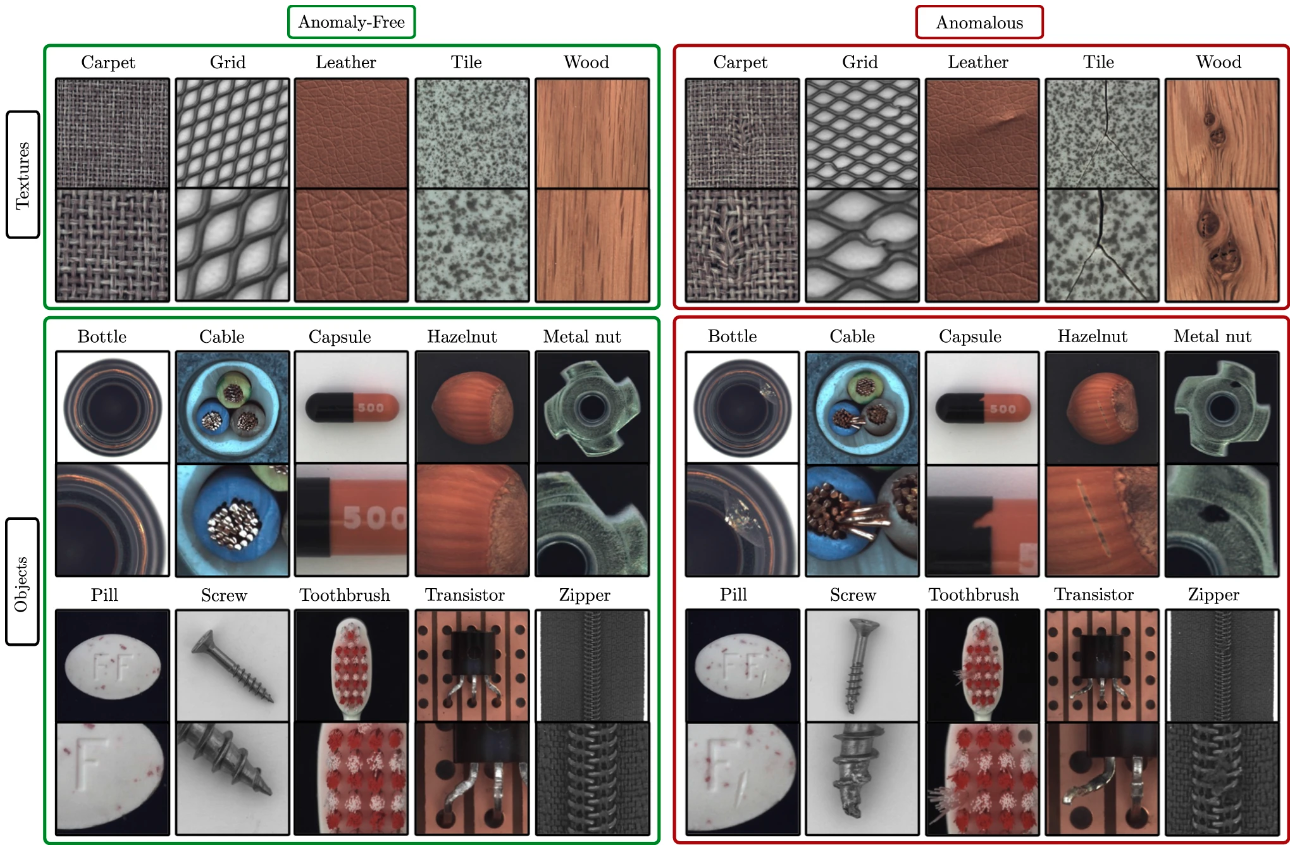
\includegraphics[width=0.95\textwidth]{bilder/mvtecad_examples.png}
  \caption{Beispiele für nominale und anomale Bilder aus dem MVTec AD Datensatz}
  \label{fig:mvtecad_examples}
\end{figure}


\section{Eigener Datensatz (Granulat)}\label{sec:EigenerDatensatz}
Details und Beispiele zu eigenem Datensatz.

\section{AUROC\cite{aurcoc}}\label{sec:AUROC}
In dieser Arbeit, genauso wie in beinahe allen anderen Arbeiten im Bereich der binären Anomalieerkennung, wird die \glqq Area Under the Receiver Operating Characteristic Curve\grqq{} (AUROC) als Leistungsmaß verwendet.\ 
Die AUROC ist ein Maß für die Fähigkeit eines binären Klassifikators, zwischen zwei Klassen zu unterscheiden. \
Nachfolgend wird schrittweise zum Begriff des AUROC hingeführt. \
\subsection{Logistische Regression}\label{subsec:LogistischeRegression}
%Die logistische Regression ist eine Methode zur binären Klassifizierung, bei der das Ziel darin besteht, ein binäres Ergebnis auf der Grundlage einer Reihe von Eingabemerkmalen vorherzusagen. \
%Bei der logistischen Regression gibt ein statistisches Modell einen Wahrscheinlichkeitswert zwischen 0 und 1 aus, der als die Wahrscheinlichkeit der positiven Klasse interpretiert werden kann. Um eine binäre Vorhersage \ 
%zu treffen, wird ein Schwellenwert auf den Wahrscheinlichkeitswert angewandt, so dass Werte oberhalb des Schwellenwerts als positiv und Werte unterhalb des Schwellenwerts als negativ eingestuft werden. \
Die logistische Regression ist eine Art verallgemeinertes lineares Modell, das üblicherweise für binäre Klassifizierungsprobleme verwendet wird. \ 
Bei der logistischen Regression besteht das Ziel darin, die Wahrscheinlichkeit eines binären Ergebnisses (z. B. nominal oder anomal) auf der Grundlage einer Reihe von Eingangsmerkmalen vorherzusagen. \ 
Das logistische Regressionsmodell verwendet eine logistische Funktion (\glqq Sigmoidfunktion\grqq{}), um die Eingabemerkmale auf die vorhergesagte Wahrscheinlichkeit abzubilden. \

Die logistische Funktion ist definiert als: \
$$ 
\sigma(z) = \frac{1}{1 + e^{-z}} 
$$

wobei $z$ eine lineare Kombination aus den Eingangsmerkmalen und ihren zugehörigen Gewichten ist: \

$$ 
z = \beta_0 + \beta_1 x_1 + \beta_2 x_2 + \cdots + \beta_p x_p 
$$

Dabei ist $\beta_0$ der Bias-Term und $\beta_1, \beta_2, \ldots, \beta_p$ sind die Koeffizienten für die Eingangsmerkmale $x_1, x_2, \ldots bzw. x_p$.

Das logistische Regressionsmodell wird trainiert, indem eine Verlustfunktion minimiert wird, die die Differenz zwischen den vorhergesagten Wahrscheinlichkeiten \ 
und den wahren binären Kennzeichnungen misst. Eine gängige Verlustfunktion für logistische Regression ist der binäre Kreuzentropie (\glq Cross-Entropy\grqq{}), die wie folgt definiert ist: \

$$ 
\mathcal{L}(\beta) = -\frac{1}{n} \sum_{i=1}^n y_i \log(\hat{y}_i) + (1 - y_i) \log(1 - \hat{y}_i)
$$

wobei $\beta$ die Modellparameter (d.h. den Achsenabschnitt und die Koeffizienten) darstellt, $n$ die Anzahl der Trainingsbeispiele, \ 
$y_i$ das wahre binäre Label für das $i$-te Beispiel und $\hat{y}_i$ die vorhergesagte Wahrscheinlichkeit für das $i$-te Beispiel ist. \

Das logistische Regressionsmodell kann mithilfe des Gradientenabstiegs trainiert werden, bei dem die Modellparameter iterativ in Richtung des negativen Gradienten der Verlustfunktion \ 
aktualisiert werden. Der Gradient der Verlustfunktion in Bezug auf die Modellparameter kann mithilfe der Kettenregel der Infinitesimalrechnung berechnet werden. \
\cite{bishop2006pattern} (Kapitel 4) \cite{intoStatLearn}
\subsection{Konfusionsmatrix}\label{subsec:Konfusionsmatrix}
Die Konfusionsmatrix ist eine Tabelle, die die Leistung eines binären Klassifikationsmodells zusammenfasst. Sie besteht aus vier Einträgen: wahr-positive (TP), falsch-positive (FP), wahr-negative (TN) und falsch-negative (FN). \ 
TP und TN stehen für die Anzahl der richtig klassifizierten positiven bzw. negativen Beispiele, während FP und FN für die Anzahl der falsch klassifizierten positiven bzw. negativen Beispiele stehen.
\begin{table}[h]
  \centering
  \begin{tabular}{|c|c|c|}
  \hline
   & \textbf{Tatsächlich Positive} & \textbf{Tatsächlich Negative} \\
  \hline
  \textbf{Prädizierte Positive} & Wahre Positive (TP) & Falsche Positive (FP) \\
  \hline
  \textbf{Prädizierte Negative} & Falsche Negative (FN) & Wahre Negative (TN) \\
  \hline
  \end{tabular}
  \caption{Konfusionsmatrix}
  \label{tab:Konfusionsmatrix}
\end{table}

Hier stehen die Zeilen für die vorhergesagten Kennzeichnungen und die Spalten für die wahren Kennzeichnungen. Die Einträge in der Diagonale stehen für die richtigen Vorhersagen, \ 
während die Einträge außerhalb der Diagonale die falschen Vorhersagen darstellen. \
Die \glqq True Positive Rate\grqq{}(TPR), die auch als Sensitivität oder Recall bezeichnet wird, ist definiert als TP / (TP + FN), d. h. der Anteil der positiven Beispiele, die richtig klassifiziert \ 
wurden. Die \glqq False Positive Rate\grqq{} (FPR) ist definiert als FP / (FP + TN), d. h. der Anteil der negativen Beispiele, die falsch klassifiziert werden. \
Die Konfusionsmatrix bietet eine Möglichkeit, die Leistung eines binären Klassifikationsmodells im Hinblick auf seine Fähigkeit, positive und negative Beispiele richtig zu klassifizieren, \ 
zu bewerten. Sie kann zur Berechnung verschiedener Leistungsmetriken verwendet werden, wie z. B. Genauigkeit, Präzision, Wiedererkennung, F1-Score und die Fläche unter der \glqq Receiver Operating Characteristic\grqq{} (ROC)-Kurve (AUC), \ 
die im nächsten Abschnitt erläutert wird.
\subsection{ROC-Kurve}\label{subsec:ROC-Kurve}
Die Receiver-Operating-Characteristic-Kurve (ROC-Kurve) ist eine grafische Darstellung der Leistung eines binären Klassifikationsmodells, wenn der Schwellenwert variiert wird.\ 
In der ROC-Kurve wird die Rate der richtig positiven Beispiele (TPR) \ 
gegen die Rate der falsch positiven Beispiele (FPR) für verschiedene Schwellenwerte aufgetragen. Die TPR ist der Anteil der positiven Beispiele, die richtig klassifiziert werden, \ 
während die FPR der Anteil der negativen Beispiele ist, die falsch klassifiziert werden. \\
Berechnet man die Fläche unter der ROC-Kurve erhält man das \textbf{\glqq Area Under the Curve\grqq{} (AUC)} Maß. Es ist eines der aussagekräftigsten Maße, die es für eine binäre Klassifikation \
wie die Anomalieerkennung gibt. Die AUC ist ein Wert zwischen $0$ und $1$, wobei $1$ für eine perfekte Klassifikation steht, $\num{0,5}$ für eine zufällige Klassifikation und $0$ für eine gänzlich falsche Klassifikation steht. \
Nachfolgend sind mögliche Ausbabeverteilungen einer logistischen Regression, markiert mit der tatsächlichen Klassenzugehörigkeit, skizziert. Diese Veranschaulichen den Zusammenhang zwischen der Ausgabe einer logistischen Regression, \
der ROC-Kurve und dem AUROC-Maß.
\newcommand{\thiswidth}{0.8\textwidth}
\begin{figure}[h]
  \centering
  \begin{subfigure}[b]{\thiswidth}
      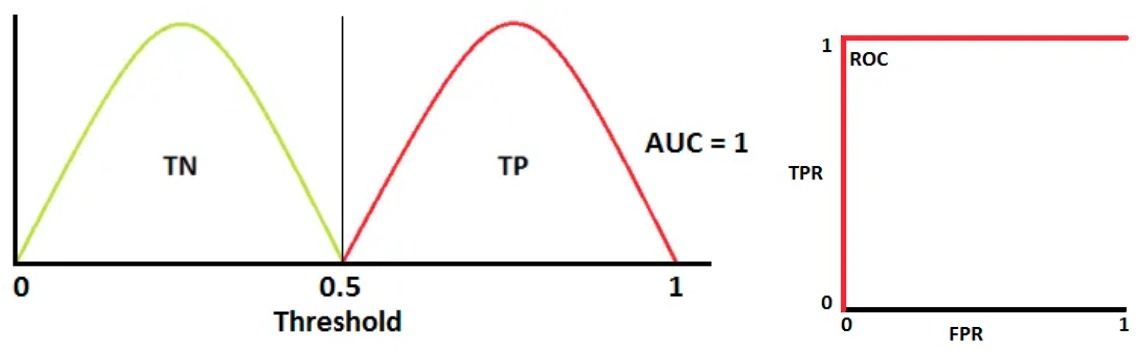
\includegraphics[width=\linewidth]{bilder/auc_1.png}
      \caption{$\mathbf{AUC = \num{100}\%}$: Die beiden Verteilungen der Klassen sind vollständig getrennt. Eine perfekte Klassifikation ist möglich.}
      \label{fig:subfig1}
  \end{subfigure}
  \hfill
  \begin{subfigure}[b]{\thiswidth}
      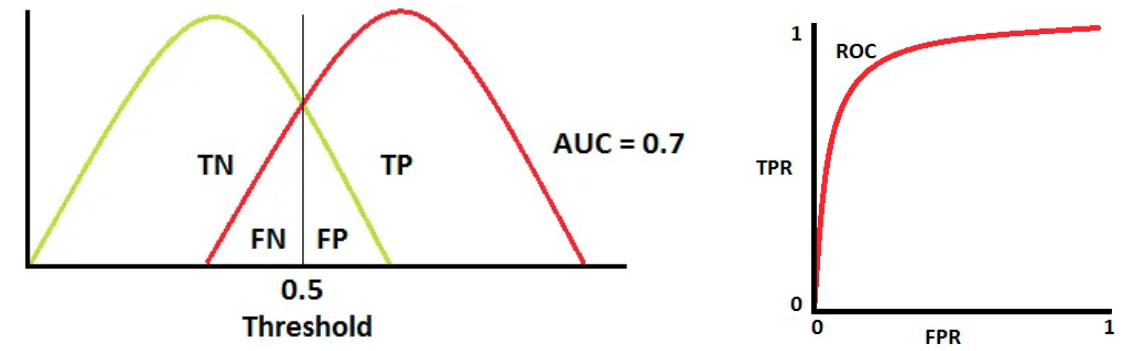
\includegraphics[width=\linewidth]{bilder/auc_07.png}
      \caption{$\mathbf{AUC = \num{70}\%}$: Eine Überlappung der Verteilungen lässt mit keinem Schwellwert eine fehlerfreie Klassifikation zu. Ein Großteil der Beispiele kann aber richtig klassifiziert werden.}
      \label{fig:subfig2}
  \end{subfigure}
  
  \begin{subfigure}[b]{\thiswidth}
      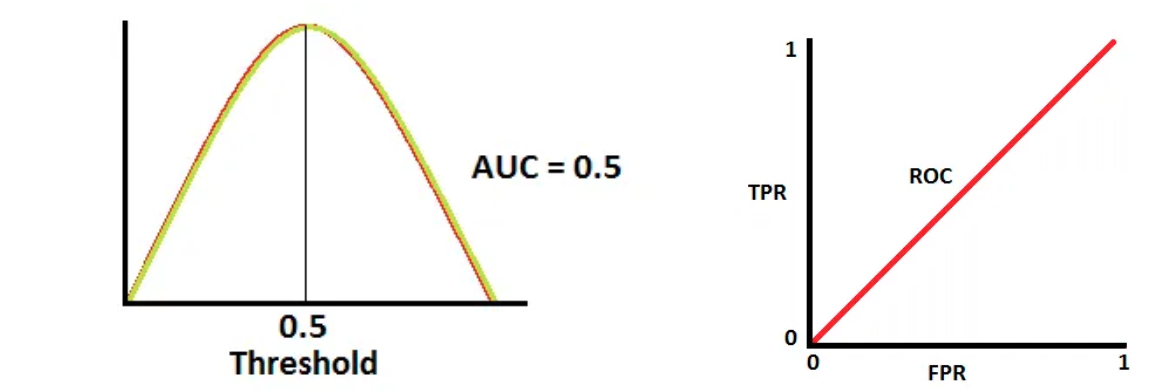
\includegraphics[width=\linewidth]{bilder/auc_05.png}
      \caption{$\mathbf{AUC = \num{50}\%}$: Die Verteilungen der Klassen überlappen sich vollständig. Eine sinnvolle Klassifikation ist somit nicht möglich. Eine Zuordnung würde zufällig geschehen.}
      \label{fig:subfig3}
  \end{subfigure}
  \hfill
  \begin{subfigure}[b]{\thiswidth}
      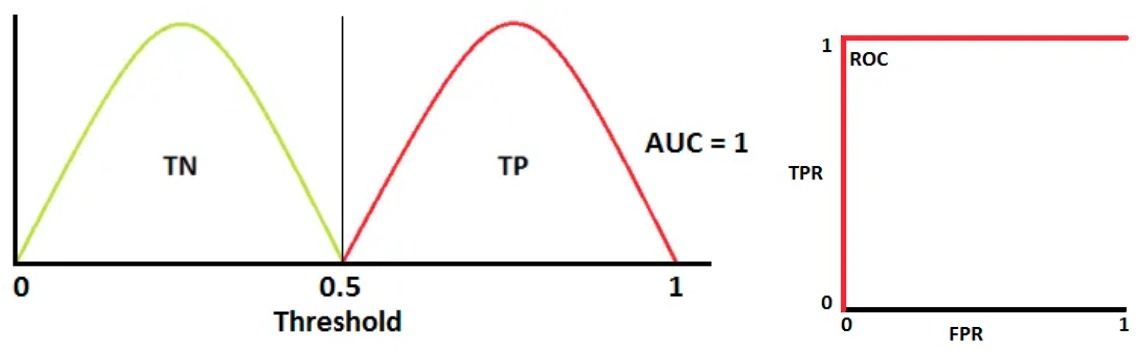
\includegraphics[width=\linewidth]{bilder/auc_1.png}
      \caption{$\mathbf{AUC = \num{0}\%}$: Dieser Spezialfall lässt keine korrekte Klassifikation zu, obwohl die Klassen eindeutig getrennt sind. Dies liegt daran, dass die Verteilung der positiven Klasse vollständig links von der Verteilung der negativen Klasse liegt. Durch eine geeignete Abbildung kann dieses Problem gelöst werden.}
      \label{fig:subfig4}
  \end{subfigure}
  \caption{Veranschaulichung verschiedener Verteilungen positiver und negativer Klassen und den dazugehörenden ROC-Kurven und AUC-Werten.}
  \label{fig:main}
\end{figure}
% \newpage
% \section{PyTorch}\label{sec:PyTorch}
% Die Implementierung dieser Arbeit geschieht mit der Programmiersprache \textbf{Python}. An dieser Stelle wird zwar mit dem Hinweis auf unzählige Literatur und Tutorials auf die Sprache Python verwiesen, \
% eine ausführliche Beschreibung würde den Rahmen dieser Arbeit überschreiten. \\
% Hingegen folgt eine Beschreibung des Frameworks \textbf{PyTorch}, das in dieser Arbeit verwendet wird. \\
% PyTorch ist ein Open-Source-Framework für maschinelles Lernen, das von Facebooks AI Research Lab (FAIR) entwickelt wurde. Es hat sich zu einem wichtigen Akteur in der \ 
% Welt der künstlichen Intelligenz und des maschinellen Lernens entwickelt. PyTorch \ 
% zeichnet sich durch Flexibilität, dynamische Berechnungsgraphen und eine benutzerfreundliche Python-Schnittstelle aus.\\
% PyTorch wird somit häufig zum 
% Im Kern zeichnet sich PyTorch durch die Entwicklung und das Training tiefer neuronaler Netze aus, was es zur ersten Wahl \\ 
% für Aufgaben wie Bild- und Spracherkennung, Verarbeitung natürlicher Sprache und Reinforcement Learning macht. Sein dynamischer Berechnungsgraph ermöglicht im Gegensatz zu statischen Graphen in Frameworks wie TensorFlow dynamische Anpassungen der Modellarchitektur während der Laufzeit. Dieser dynamische Ansatz ist besonders für die Forschung von Vorteil, da er das Experimentieren und die Modellentwicklung vereinfacht.

% Darüber hinaus nutzt PyTorch Hardware-Beschleunigung, einschließlich GPU-Unterstützung, was den Trainingsprozess dramatisch beschleunigt und es zu einer ausgezeichneten Wahl für große Projekte macht.

% Das Framework verfügt über ein reichhaltiges Ökosystem von Bibliotheken und Modulen, die die Erstellung komplexer neuronaler Netze erleichtern. Bemerkenswerte Bibliotheken wie TorchVision und TorchText erleichtern Aufgaben der Computer Vision bzw. der Verarbeitung natürlicher Sprache, während andere sich auf Reinforcement Learning und generative Modellierung konzentrieren.

% PyTorch hat eine treue Gemeinschaft von Nutzern und Mitwirkenden gewonnen, die seine Fähigkeiten aktiv verbessern, seine umfangreiche Dokumentation pflegen und in Foren und Diskussionen Hilfe anbieten. Diese starke Unterstützung durch die Gemeinschaft hat dazu beigetragen, dass sich PyTorch schnell weiterentwickelt und an die aufkommenden Trends in der Deep Learning- und KI-Forschung angepasst werden konnte.

% In den letzten Jahren ist die Popularität von PyTorch sprunghaft angestiegen und hat sowohl in der Wissenschaft als auch in der Industrie Anklang gefunden. Forscher bevorzugen den forschungsorientierten Ansatz, während Unternehmen die Flexibilität und die produktionsreifen Funktionen schätzen. Die Beiträge von PyTorch zu den Fortschritten in der KI sind in zahlreichen hochmodernen Modellen und Forschungsarbeiten in verschiedenen Bereichen zu finden.
\section{Residuale Netzwerke}\label{sec:ResidualNetworks}
In diesem Abschnitt werden die Grundlagen von Residual Networks (textbf{\glqq ResNets\grqq{}}) erläutert. \
Diese spielen für die Merkmalsextraktoren (\glqq Feature Extractors\grqq{}) in den im Haupteil der Arbeit (TODO --> Link) eine wichtige Rolle. \
Der Schwerpunkt hierbei liegt auf der grundlegenden Idee, der Rolle, die ResNets historisch in der Entwicklung von Deep Learning gespielt haben und \
vor allem den Aspekten, die für die Anwendung in dieser Arbeit relevant sind. \ 
Für detailierte Informationen zu ResNets wird auf das Paper von Kaiming He et al. \cite{resnet} und die zahlreichen Erläuterungen in der Literatur verwiesen. \
\subsection{Hintergrund \& Idee hinter \glqq ResNets\grqq{}}\label{subsec:ResNetsBackgroundAndIdea}
Tiefe neuronale Netze (Deep Neural Networks, DNNs) eignen sich hervorragend für das Lernen hierarchischer Darstellungen aus Daten,\
aber sie stehen vor Herausforderungen, wenn sie \glqq tiefer\grqq{} werden.\glqq Tiefe\grqq{} bezeichnet in diesem Zusammenhang \ 
die Anzahl an Schichten, die sequentiell durchlaufen werden, um das Endergebnis bzw. die Ausgabe zu erhalten. \
Tiefere Netze können komplexere Merkmale in Daten erfassen, was für Aufgaben wie die Bildklassifizierung, bei der Objekte und Muster komplizierte Details aufweisen können, entscheidend ist.\
Einer der großen Herausforderungen bei tiefen Netzen ist das Problem der \glqq verschwindenden Gradienten\grqq{} (\textit{engl.} \textbf{Vanishing Gradients}). \
Diese Gradienten sind entscheidend für das Training eines Neuronalen Netzes, insofern, als dass das Optimierungsverfahren des Gradientenabstiegs die Grundlage auch moderner Optimierer wie \glqq Adam\grqq{} (TODO --> Ref) ist. \ 
Dieses Problem lässt sich anschaulich dadurch erklären, dass frühe Gradienten, was sich leicht mithilfe der Kettenregel zeigen lässt, \ 
eine Multiplikation von allen nachfolgenden (im Sinne der Infernenzrichtung - \glqq forward pass\grqq{}) Gradienten darstellt. \
Betrachtet man nun ein sehr tiefes Netz, das heißt, viele Gradienten, die miteinander multipliziert werden und den wahrscheinliche Fall von Gradienten, die kleiner als $1$ sind, so wird schnell klar, dass frühe Schichten einen sehr kleinen Gradienten haben können. \
Dies macht es schwierig, die Gewichte der frühen Schichten zu aktualisieren, was den Lernprozess behindert. Dabei ist es vor allem die Tiefe, die Neuronalen Netzen das Generalisieren von komplexen Zusammenhängen ermöglicht (\glqq Deep Learning \grqq{})\\
Residuale Netze, allgemein bekannt als ResNets und im Folgenden auch so bezeichnet, wurden von Kaiming He et al. (TODO --> Ref) in ihrem Paper von 2015 vorgestellt und bieten eine einfache und dennoch effektive Methode an, wie dieses Problem angegangen werden kann. \
Die Grundidee besteht darin, Verknüpfungen zwischen den Schichten einzuführen, die es dem Netz ermöglichen, eine oder mehrere Schichten zu \glqq überspringen\grqq{}. \ 
Anstatt die gewünschte Abbildung also direkt zu lernen, lernen ResNets die residuale Abbildung, was der Differenz zwischen Ein- und Ausgabe entspricht. Die Eingabe wird über sogenannte \
\glqq Shortcut (Skip) Connections\grqq{}, also einfach die Identitätsabbildung, vom Eingang zur residualen Ausgabe weitergeleitet, um dann durch Summation wieder miteinander verknüpft zu werden. \
Das Problem der verschwindenden Gradienten wird dadurch entschärft, dass die Gradienten direkt in frühere Schichten zurückfließen können. 
Anschaulich lässt sich das durch die Tatsache erklären, dass die Identitätsabbildung einen konstanten Gradienten von $1$ besitzt. Weil sich die Summenbildung \
am Ausgang eines nachfolgend noch im Detail besprochenen Residual-Blocks auch bei der Gradientenbildung als Summation widerspiegelt, ist der Gradient einer jeden Schicht nicht mehr das Produkt, sondern vielmehr die Summe aller nachfolgenden Gradienten. (Optional TODO: Formel) 
Das zugrundeliegende Paper ist eines der meistzitierten Paper im Bereich des Deep Learning und hat die Entwicklung von Deep Learning maßgeblich beeinflusst. \
\subsection{Residual Block \& Architektur}\label{subsec:ResidualBlocks}
Der Grundbaustein eines ResNet ist der Residualblock. Er besteht aus zwei Hauptpfaden: dem Identitätspfad (der Abkürzungsverbindung) und dem Residualpfad (dem Hauptfaltungspfad).\ 
Mathematisch wird die Ausgabe eines Residualblocks wie folgt berechnet:
\[
\text{Output} = F(\text{Input}) + \text{Input}
\]
wo $F$ die Residualabbildung ist, die durch die Hauptfaltungsschichten gelernt wird.\  
%The shortcut connection allows the gradients to flow directly back to earlier layers without vanishing, making it easier for the network to learn.
Nachfolgende Abbildung zeigt eine vereinfachte Darstellung eines \glqq Building Blocks\grqq{} bzw. Residual Block. \
\begin{figure}[H]
  \centering
  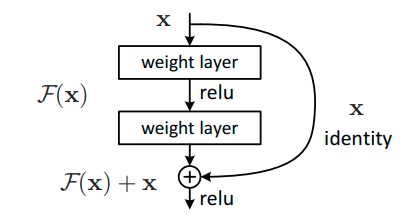
\includegraphics[width=0.5\textwidth]{bilder/residual_block.png}
  \caption{Residual Block (TODO --> Ref)}
  \label{fig:ResidualBlock}
\end{figure}
Ein ResNet besteht aus mehreren Residualblöcken, die sequentiell durchlaufen werden. Es ist also eine \glqq Feed-Forward\grqq{}-Architektur, weil die Daten zur Inferenz \ 
nur in eine Richtung durch das Netz fließen. Durch das \glqq Stapeln \grqq{} können dann sehr tiefe Netze erstellt werden, die sich dennoch aufgrund der oben beschriebenen
Eigenschaften gut optimieren bzw. trainieren lassen. \\
Es existieren zahlreiche verschiedene Varianten von ResNets, die sich in der Art und Anzahl ihrer Residual Blöcke unterscheiden. \
Nachfolgende Tabelle gibt einen Überblick über die drei, in dieser Arbeit vor allem verwendeten Varianten: ResNet18, ResNet34 und WideResNet50 \

\begin{table}[h]
  \centering
  \begin{tabular}{|c|c|c|c|c|}
  \hline
  \textbf{Netzwerk} & \textbf{Tiefe} & \textbf{\# Parameter} & \textbf{Top-1 Fehlerrate\tablefootnote{in ILSVRC (TODO --> Ref)}} & \textbf{Inferenz auf RBP4\tablefootnote{Raspberry Pi 4B 8GB. Betrachtet wurde die Laufzeit von einem Bild der Auflösung 224x224 und 3 (Farb-)Kanälen}} \\ \hline
  ResNet18         & \makecell{$18$}             & \makecell{$\num{11,7e6}$}                        & \makecell{$\num{30.24}$\%}                   & \makecell{$0,82\si{\second}$}\\ \hline
  ResNet34         & \makecell{$34$}             & \makecell{$\num{21,8e6}$}                       & \makecell{$\num{26.70}$\%}                   & \makecell{$1,45\si{\second}$}\\ \hline
  WideResNet50     & \makecell{$50$}             & \makecell{$\num{68,9e6}$}                        & \makecell{$\num{22.53}$\%}                   & \makecell{$3,00\si{\second}$}\\ \hline
  \end{tabular}
  \caption{Vergleich verschiedener ResNet Varianten (TODO --> Ref)}
  \label{tab:resnet-comparison}
\end{table}
Zu erkennen ist eindeutig, dass die Anzahl der Parameter und die Inferenzzeit mit der Tiefe des Netzes steigt. \
Gleichzeitig lässt sich aber auch eine Verbesserung der Top-1 Fehlerrate erkennen, je tiefer bzw. mächtiger das Netz ist. \\
Einer der Hauptvorteile von ResNets ist die Fähigkeit, Merkmale pyramidenförmig durch das Netz zu verbreiten. Das bedeutet, dass das Netz Merkmale auf verschiedenen \ 
Abstraktionsebenen erfassen kann, von Low-Level-Merkmalen wie Kanten und Ecken bis zu High-Level-Merkmalen wie Objektteilen und semantischen Konzepten. \
Mit zunehmender Tiefe wird also die Auflösung der \glqq Feature Maps\grqq{} (TODO --> Ref) reduziert, während die Anzahl der Kanäle und die Komplexität der zugrundeliegenden Merkmale zunimmt. \
Dargestellt ist das in folgender Abbildung:
\begin{figure}[H]
  \centering
  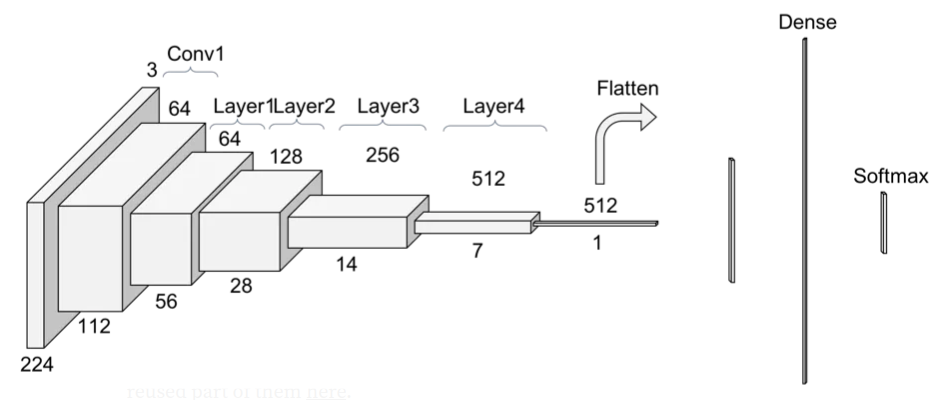
\includegraphics[width=0.8\textwidth]{bilder/resnet_pyramid.png}
  \caption{Pyramidale Merkmalsverteilung in ResNets (TODO --> Ref)}
  \label{fig:ResNetPyramid}
\end{figure}
Die Quader in oben stehendem Netz stehen symbolhaft für die Auflösung der Feature Maps. \
Während die oben stehenden Zahlen die Anzahl der Kanäle repräsentieren, stehen die unten aufgeführten Zahlen für die räumliche Auflösung. Letztere hängt \ 
proportional von der Auflösung des Eingangsbildes ab und gilt für alle drei Modelle. Die Anzahl an Kanälen ist konstant für alle Auflösungen und für ResNet18 und ResNet34. \
Für das WideResNet50 gilt im Wensentlichen der gleiche Aufbau, allerdings sind die Kanäle \glqq geweit\grqq{} gegenüber den anderen beiden Architekturen, was \
sich an der Vervierfachung der Anzahl an Kanäle durch Verwendung eines komplexeren Residual Blocks (\glqq Bottleneck\grqq{}\cite{wideresnet})zeigt. 
ResNet18 und ResNet34 unterscheiden sich ausschließlich in der Anzahl der Residual Blöcke bzw. der Tiefe des Netzes. \\
Alle der drei hier vorgestellten Architekturen lassen sich in fünf Faltungsschichten (\glqq Conv1\grqq{}, \glqq Layer1\grqq{}, \glqq Layer2\grqq{}, \glqq Layer3\grqq{}, \glqq Layer4\grqq{}) unterteilen. \
Dem schließt sich eine \glqq Average Pooling\grqq{}-Schicht an, die die Auflösung der Feature Maps auf 1 reduizert (\glqq Flatten\grqq{}). Dieser 1D-Vektor wird \
schließlich durch eine \glqq Fully Connected\grqq{}-Schicht (\glqq Dense\grqq{}) auf die Anzahl der Klassen (1000) abgebildet. Schließlich wird durch eine \glqq Softmax\grqq{}-Aktivierungsfunktion \
Pseodo-Wahrscheinlichkeiten erzeugt, die den Axiomen von Kolmogorov entsprechen und somit als Auftrittswahrscheinlichkeiten interpretiert werden können.\\
In dieser Arbeit werden die ResNets als Feature-Extraktoren verwendet, weshalb die letzten beiden Schichten, also \glqq Flatten\grqq{} und \glqq Dense\grqq{} nicht verwendet werden. \ 
Die Begriffe \glqq Layer1 - Layer4\grqq{} werden im Folgenden in dem hier beschriebenen Kontext verwendet. \\ 
\subsection{ResNets as Feature Extractor für Unüberwachte Lernverfahren}\label{subsec:ResNetsAsFeatureExtractor}
Zusätzlich zu ihrem Erfolg bei der überwachten Bildklassifizierung haben ResNets Anwendungen als leistungsstarke Merkmalsextraktoren bei Unüberwachten Klassifizierungsaufgaben \ 
wie der Anomalieerkennung gefunden. In unüberwachten Szenarien wie der Anomalieerkennung stehen oft keine markierten (gelabelten) Daten zur Verfügung, wie bereits in \ref{sec:UnueberwachteAnomaliedetektion} beschrieben, um ein Modell explizit bzw. überwacht zu trainieren. \ 
Stattdessen verlässt man sich auf das Lernen von Darstellungen normaler Daten und identifiziert dann Abweichungen als Anomalien. ResNets können mit ihrer Fähigkeit, umfangreiche und hierarchische Merkmale \ 
zu erfassen, dazu verwendet werden, sinnvolle Merkmale aus den Daten zu extrahieren. Es kann mithilfe dieser Netze eine kompaktere und aussagekräftigere Darstellung der Daten erzeugt werden, die die Grundlage sind, \
um auch komplexere Anomalien zu erkennen. Allerdings ist festzuhalten, dass die extrahierten Feature in keiner Weise optimiert sind, um Anomalieklassifikationen zu ermöglichen, sondern um auf dem ImageNet-Datensatz \
Bilder richtig einzuordnen. Vor allem in späteren Schichten ist also zu erwarten, dass die Merkmale einene \glqq Bias \grqq{} hin zu ImageNet aufweisen, der sich negativ auf die Anomalieklassifikation auswirken kann.\cite{patchcore} \ 
Hierzu werden die Gewichte offizieller Implementierungen von ResNets verwendet, womit das eigentliche Vortraining \ 
entfällt und Reproduzierbarkeit, Konsistenz und Vergleichbarkeit der Ergebnisse gewährleistet wird. \\
Alle hier vorgestellten Methoden verwenden ResNets als Feature-Extraktoren, wenn auch im Ansatz\glqq EffientAD\grqq{} (\ref{ch:EfficientAD}) nicht während der Inferenz. \
Gezeigt, dass eine solche Feature Extraktion im Kontext der Unüberwachten Anomalieerkennung sinnvoll ist, wurde erstmals in der Veröffentlichung\glqq Deep Nearest Neighbor Anomly Detection\grqq{} von Bergman et al.\cite{DN2} mit der Methode \glqq DN2\grqq{} im Februar 2020. \
Im nachfolgenden Abschnitt wird die darauf aufbauende Methode \glqq SPADE\grqq{}, vom gleichen Team entwickelt, vorgestellt. \
% \section{Autoencoder}\label{sec:Autoencoder}
% Hier kommt dann eine relativ generische Erläuterung von Autoencodern. \
% Gefolgt von Autoencoder für Anomaliedetektion. \
\section{SPADE}\label{sec:SPADE}
Die Methode \textbf{SPADE} ist ein wichtiger Meilenstein in der Unüberwachten Anomalieerkennung.\
Zahlreiche erfolgreiche Methoden bauen auf SPADE auf und übernehmen wichtige Elemente und Konzepte.\
Das Paper wurde am 5. Mai 2020 von Niv Cohen und Yedid Hoshen von der Hebräischen Universität von Jerusalem veröffentlicht.\
Im Folgenden wird SPADE vorgestellt.\
\subsection{Funktionsweise}\label{subsec:SPADEFunktionsweise}
\subsubsection*{Feature Extraktion}
Wie bereits in \ref{subsec:ResNetsAsFeatureExtractor} beschrieben, werden ResNets erfolgreich als Feature-Extraktoren verwendet.\
Der Name \glqq SPADE\grqq{} steht hierbei für \glqq Semantic Pyramid Anomaly Detection\grqq{}. Betrachtet man \ref{fig:ResNetPyramid} wird klar warum von einer \glqq Pyramide\grqq{} gesprochen werden kann:\
Es werden die Feature Maps der einzelnen Schichten, konkret der Schichten \glqq Layer1, Layer2 und Layer3\grqq{} als Feature unverändert verwendet.\
Dabei wird auf einen Einbettungsprozess, wie bei anderen Methoden üblich, verzichtet.\ Durch die mit der Tiefe des Netzes abnehmende Auflösung der Feature Maps, \
entsteht so eine \glqq Pyramidale\grqq{} Struktur, die eben die Grundlage für die Namensgebung ist.\
Zusätzlich wird der 1D-Vektor, der durch die \glqq Flatten\grqq{}-Schicht erzeugt wird, als Feature verwendet, um instanzweise, also für jedes Bild als Ganzes, zu entscheiden, ob eine \
Anomalie vorliegt, wie im nächsten Abschnitt beschrieben.\
Bezeichnen wir das ResNet als Feature-Extraktor mit $F$, so lassen sich die Feature $f_{i}$ eines gegebenen Bildes $x_{i}$ wie folgt beschreiben:
$$f_{i} = F(x_{i})$$
In der Trainings- bzw. Initialisierungsphase werden die Feature $f_{i}$ aller Trainingsbilder $x_{i}$, welche alle nominal sind, extrahiert und gespeichert.\
Diese Menge wird im Folgenden mit $F_{train}$ bezeichnet.\
\subsubsection*{Instanzklassifizierung}
Die Instanzklassifizierung ist der zweite Schritt von SPADE. Es wird dabei für jedes Bild $y_{i}$ aus der Menge an Testbilder $Y$ entschieden, ob es sich um eine Anomalie handelt oder nicht.\
Dies geschieht ausschließlich anhand des 1D-Vektors, der durch die \glqq Flatten\grqq{}-Schicht erzeugt wird.\
Hierzu wird für ein gegebenes Testbild $y_{i}$, die $K$ nächsten Nachbarn in $F_{train}$ gesucht. Diese Menge an $K$ Vektoren wird fortan als $N_{k}(f_{y})$ bezeichent. \
Es wird eine Distanz auf die folgende Art und Weise bestimmt:
$$
d(y_{i}) = \frac{1}{K} \sum_{f\in N_{k}(f_{y_{i}})} \left|\left| f - f_{y_{i}} \right|\right|^{2}
$$
Die Distanz $d(y_{i})$ wird dann mit einem Schwellenwert $\tau$ verglichen. Ist die Distanz kleiner als der Schwellenwert, so wird das Bild als nominal klassifiziert, ansonsten als Anomalie.\
\subsubsection*{Segmentierung}
Nachdem eine Instanzklassifiziergung ergeben hat, dass es sich um ein anomales Bild handelt, besteht die nächste Aufgabe darin, die Anomalie oder mehrere Anomalien auf dem Bild zu lokalisieren.\
Dieser Schritt wird übersprungen, wenn das Bild als nominal klassifiziert wurde.\\
Die naive Methode, die Anomalie zu lokalisieren, wäre es, die Differenz zwischen dem anomalen Bild und dem ausgerichtete Bild des nächsten Nachbarn zu berechnen. Dort, wo die Differenz am größten ist, \
wird die Anomalie vermutet. Allerdings hat diese Methode einige Schwachstellen. Zum einen kann die Ausrichtung des nächsten Nachbarn so, dass das zu untersuchende Objekt im Bild an der gleichen Stelle ist, \
fehlschlagen. Insbesondere. Auch kann insbesondere bei eienem kleinen Datensatz und Objekten, die komplexe Variationen aufweisen möglicherweise kein passender Nachbar gefunden werden, was zu falsch positiven (anomalen) \
Klassifizierungen führen kann. Außerdem könnte die Berechnung der Differenz sehr empfindlich auf die verwendete Berechnungsmethode sein.(TODO... Vllt einfach weg lassen?)\\ 
Um diese Probleme zu überwinden, wird eine Übereinstimmungsmethode präsentiert, die mit vielen \glqq Bildern\grqq{} arbeitet (\glqq multi-image correspondence method\grqq{}). Diese Bilder entsprechen den Feature Maps der Schichten Layer1, Layer2 und Layer3, \
also gewissermaßen den Quader in \ref{fig:ResNetPyramid}.\\
Nun gilt es zu jeder Pixelposition $p\in P$ die korresponierenden Feature $F(x_{i}, p | p\in P)$ zu bestimmen. Auf jedes Bild aus dem Trainingsdatensatz $x_{i}$ \ 
angewandt und ergibt sich dann die \glqq Gallerie\grqq{} zu $G = \{ {F(x_{1}, p | p\in P)}\cup {F(x_{2},p|p\in P)} .. \cup {F(x_{K},p|p\in P)} \}$.\\
Der Anomaliegrad eines Pixels $p$ ist dann gegeben durch die durchschnittliche Distanz zwischen dem Feature $F(y_{i},p)$ des anomalen Bildes $y_{i}$ und \ 
den $\kappa$ nächsten Featuren aus der Gallerie $G$. Es ergibt sich also für einen Pixel $p$ im Testbild $y_{i}$ folgende Formel: \
$$
d(y_{i},p) = \frac{1}{\kappa} \sum_{f\in N_{\kappa}(F(y_{i},p))} \left|\left| f - F(y_{i},p) \right|\right|^{2}
$$
Für einen gegebenen Schwellwert $\theta$ wird ein Pixel $p$ als anomales Pixel klassifiziert, wenn $d(y_{i},p) > \theta$ gilt.
Dies ist dann der Fall, wenn wir kein nominales Feature in $G$ finden können, welches dem Feature $F(y_{i},p)$ ausreichend ähnlich ist.\\
Dadurch, dass die Gallerie $G$ die Positionsinformation $p$ marginalisiert, wird die Segmentierung robust gegenüber der Ausrichtung. Anschaulich gesprochen, wird \
also in jedem Bild an allen Positionen nach ähnlichen Features gesucht.
\subsection{Ergebnisse und Diskussion}\label{subsec:SPADEResults}
Wie bereits erwähnt, markiert diese Arbeit einen wichtigen Entwicklungsschritt in der Forschung zur Unüberwachten Anomalieerkennung. \
Folgende Aspekte sollten in diesem Zusammenhang hervorgehoben werden:
\begin{itemize}
  \item SPADE ist die erste ganzheitliche Methode, die auf ImageNet vortrainierte ResNets als Feature-Extraktoren verwendet. Dieser Ansatz hat sich als sehr erfolgreich erwiesen und wird von zahlreichen Methoden übernommen. \
  \item Das Zusammenfassen aller extrahierten Features aus den Testbildern zu einer Menge $G$ löst das Problem der Ausrichtung und ermöglicht eine robuste Segmentierung. Auch diese Idee wird uns bei PatchCore (\ref{ch:PatchCore}) wiederbegegnen.\
  \item Das Bestimmen des Anomaliegrades mithilfe einer kNN-Suche ist ein einfacher und effektiver Ansatz, der sich auch in modifizierter Form in vielen anderen Methoden wiederfindet.\
\end{itemize}
Insbesondere in der pixelweisen Klassifikation von Anomalien hat sich SPADE als geeignet erwiesen. Auch in der Instanzklassifiziergung erreicht diese Methode auf dem damals \
noch jungen Datensatz MVTecAD gute, zum Zeitpunkt der Veröffentlichung der Methode, sogar das beste Ergebnisse.\\
Für das Ziel dieser Arbeit, welche den Fokus auf die Instanzklassifiziergung und die Laufzeitoptimierung legt, ist SPADE allerdings eher ungeeignet. \
Zum Einen sind \num{85,5}\% erreichte Bildklassifizierungsgenauigkeit auf MVTecAD für die Instanzklassifizierung nicht mit neueren, zum Teil aber auf SPADE aufbauenden Methoden, konkurrenzfähig. \
Zum Anderen ist die notwendige kNN Suche, die für jedes Testbild durchgeführt werden muss, sehr rechenintensiv. Dieser Rechenaufwand skaliert linear mit der Anzahl an Bildern im Trainingsdatensatz und mit der Anzahl der Pixel pro Bild.\
Kann man auf eine Segmentierung verzichten, verkleinert sich der Rechenaufwand zwar deutlich, es muss aber dennoch eine kNN-Suche über alle Trainingsbilder für jedes Testbild durchgeführt werden, wodurch die Laufzeit wiederum von der Größe des Trainingsdatensatz abhängt, \ 
auch wenn die Auflösung der Bilder keinen Einfluss mehr hat. \
Den Anstoß und die Impulse, die durch diese Veröffentlichung gesetzt wurden, sind jedoch nicht zu unterschätzen. \

\section{PaDiM}\label{sec:PaDiM}
Die Methode \textbf{PaDiM} wurde am 17. November 2020 von Defard et al. (Universität Paris-Saclay) veröffentlicht.\
Es werden einige Aspekte von SPADE übernommen, vor allem aber Schwächen der Methode erfolgreich addressiert. Einer der wesentlichen Unterschiede zwischen PaDiM und SPADE ist, die Weise auf die der Anomaliescore bestimmt wird. \ 
PaDiM markierte damit die beste Instanzklassifizierungsgenauigkeit auf dem Datensatz MVTecAD zum Zeitpunkt der Veröffentlichung und hielt dies bis zum Erscheinen der Methode \glqq PatchCore\grqq{}.
Nachfolgend wird der Ansatz von PaDiM vorgestellt und diskutiert.\
\subsection{Funktionsweise}\label{subsec:PaDiMFunktionsweise}
\begin{figure}[H]
  \centering
  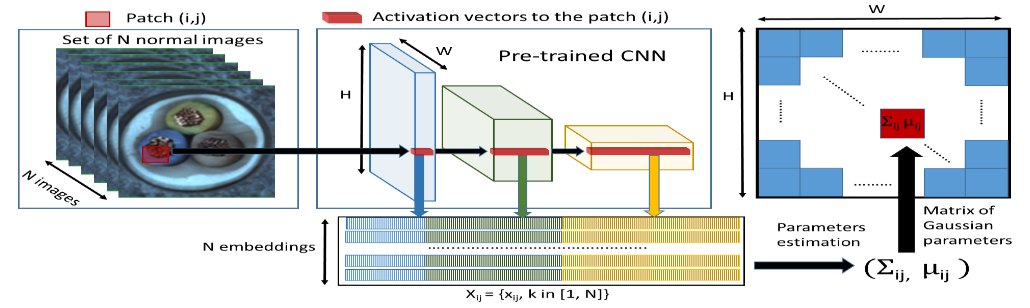
\includegraphics[width=0.8\textwidth]{bilder/padim.png}
  \caption{PaDiM: Funktionsweise (TODO --> Ref)}
  \label{fig:PaDiMOverview}
\end{figure}
% In \ref{fig:PaDiMOverview} ist die Funktionsweise von PaDiM dargestellt. \
PaDiM kann in drei Schritte unterteilt werden: \
\begin{enumerate}
  \item Feature Extraktion und Einbettungsprozess mithilfe eines vortrainierten ResNets
  \item Bestimmen der Gaußverteilungen durch Schätzen der Parameter $\mu$ und $\Sigma$ für jede Position im Bild
  \item Bestimmen des Anomaliegrades durch die Mahalanobis-Distanz
\end{enumerate}
\ref{fig:PaDiMOverview} veranschaulicht den Prozess exklusive der Inferenz. \
\subsubsection*{Feature Extraktion und Einbettungsprozess}
Der Prozess des Erzeugens von Featuren ist bei PaDiM sehr ähnlich zu dem von SPADE: \
Auch hier werden Feature Maps unterschiedlicher Auflösung und Abstraktionsebene zu einem Featurevektor zusammengefasst, der mit einer Position bzw. einem Pixel des Eingangsbildes korresponiert. \
Die Feature Map, welche die höchste Auflösung besitzt, also die Feature Map der ersten zur Feature Extraktion ausgewählten Schicht, definiert die Auflösung der Anomaliesegmentierung. \
Nehmen wir an diese Feature Map habe eine Auflösung von $W\times H$, so korresponiert also zu jeder Position $(i,j)\in [1,W]\times[1,H]$ ein Featurevektor $x_{ij}$ (\glqq Patch Embedding Vektor\grqq{}). \\
\subsubsection{Bestimmen der Gaußverteilungen}
PaDiM modelliert für jede Position eine multivariate Normalverteilung, die durch die Featurevektoren aller Trainingsbilder an dieser Position definiert wird. \\
Zunächst wird hierzu die Menge an Patch Embedding Vektoren für eine Position $(i,j)$ aus dem gesamten Trainingsdatensatz gebildet. Diese Menge \
$X_{ij} = \{ {x_{ij}^{k} | k\in [1,N]} \}$ aus den $N$ nominalen Bildern im Trainingsdatensatz wird dann benutzt, um die Normalverteilung für die Position $(i,j)$ zu bestimmen. \
Es wird also angenommen, $X_{ij}$ würde von der multivariaten Gaußverteilungen $N(\mu_{ij}, \Sigma_{ij})$ erzeugt werden. \
Die Parameter $\mu_{ij}$ und $\Sigma_{ij}$ werden dann wie folgt geschätzt: \
$$
\mu_{ij} = \frac{1}{N} \sum_{k=1}^{N} x_{ij}^{k}
$$
$$
\Sigma_{ij} = \frac{1}{N-1} \sum_{k=1}^{N} (x_{ij}^{k} - \mu_{ij})(x_{ij}^{k} - \mu_{ij})^{T} + \epsilon I
$$
wobei der Regularisierungsterm $\epsilon I$ hinzugefügt wird, um die Invertierbarkeit bzw. den vollen Rang der Kovarianzmatrix $\Sigma_{ij}$ zu gewährleisten. \
Schließlich wird die multivariate Gaußverteilung $N(\mu_{ij}, \Sigma_{ij})$ für jede Position $(i,j)$ im Bild definiert.\
\subsubsection{Bestimmen des Anomaliegrades}
Um den Anomaliegrad zu bestimmen, wird die Mahalanobis-Distanz herangezogen.%\cite{mahalanobis1936generalized} \
Die Mahalanobis-Distanz ist eine Verallgemeinerung der euklidischen Distanz, die die Korrelation zwischen den Dimensionen der Daten berücksichtigt. \
In diesem Fall lässt sich die Mahalanobis-Distanz für die Position $(i,j)$ und einem aus einem Testbild extrahierten Patch Embedding Vektor $y_{ij}$ wie folgt berechnen: \
$$
M(y_{ij}) = \sqrt{(y_{ij} - \mu_{ij})^{T} \Sigma_{ij}^{-1} (y_{ij} - \mu_{ij})}
$$
Damit kann dann eine Anomaliekarte $M$ für ein Testbild $y$ erzeugt werden:
$$
M = (M(y_{ij}))_{1<=i<=W, 1<=j<=H}
$$
Hierbei deuten hohe Werte auf eine Anomalie hin, während niedringe Werte auf einen nominalen Bildbereich hinweisen. \
Durch Maximalwerbildung über die Anomaliekarte $M$ kann dann ein Anomaliegrad $s$ für ein Testbild $y$ bestimmt werden: \
$$
s(y) = \max_{1<=i<=W, 1<=j<=H} M(y_{ij})
$$
\subsection{Ergebnisse und Diskussion}\label{subsec:PaDiMResults}
Wie bereits zu Beginn dieses Kapitels erwähnt, erreicht PaDiM zum Zeitpunkt der Veröffentlichung die beste Instanzklassifizierungsgenauigkeit auf dem Datensatz MVTecAD mit \num{97,5}\%. 
Auch die Segmentierungsergebnisse sind mit \num{97,9}\% zum Veröffentlichungszeitpunkt State-of-the-Art. \\
Ein spannender Aspekt, der in diesem Veröffentlichung untersucht wird, ist das Reduzieren der Anzahl an Kanälen bzw. die Reduzierung der Dimensionalität der Featurevektoren: \\
Es wird gezeigt, dass im Falle eines ResNet18 als Backbone die Dimensionalität von ursprünglich \num{448} auf \num{200} oder sogar \num{100} reduziert werden kann, ohne \
dass die Klassifizierungsgenauigkeit signifikant sinkt. Dabei wurden die zu entfernenden Dimensionen zufällig ausgewählt und die Ergenisse über mehrere Durchläufe gemittelt. \
Im Falle aller \num{448} Dimensionen wird eine Genauigkeit von \num{97,1}\% erreicht, während bei \num{200} Dimensionen eine Genauigkeit von \ 
\num{97,0}\% und bei \num{100} Dimensionen eine Genauigkeit von \num{96,7}\% erreicht wird. \\
Dies ist vor allem deshalb eine sehr relevante Erkenntnis, da die Reduzierung der Dimensionalität einen ganz erhebliche Einfluss auf die Berechnungsgeschwindigkeit der Mahalanobis-Distanz hat. \
Die Komplexität in der Landau-Notation für die Berechnung der Mahalanobis-Distanz zwischen zwei Vektoren der Länge $d$ ist $\mathcal{O}(d^{3})$\cite{bishop2006pattern}, \ 
wobei $d$ die Dimensionalität der Featurevektoren ist, in diesem Beispiel also \num{448}, \num{200} bzw. \num{100}. \
Dass der Einbruch der Genauigkeit bei einer Reduzierung der Dimensionalität so gering ist, ist auf die Mahalanobis-Distanz zurückzuführen, die die Korrelation zwischen den Dimensionen der Daten berücksichtigt. \
Weil die einzelnen Dimensionen teilweise stark korreliert sind, kann die Dimensionalität reduziert werden, ohne dass die Genauigkeit signifikant sinkt. \
Dies ist ein Vorteil gegenüber der euklidischen Distanz, die die Dimensionen unabhängig voneinander betrachtet, aber auch deutlich weniger komplex und damit laufzeitkritisch ist, als die \
Mahalanobis-Distanz. \\
Ein Verbesserung gegenüber SPADE ist, dass die Instanzklassifiziergung auf Grundlage der Anomaliekarte $M$ erfolgt, die durch die Maximalwerbildung über alle Positionen im Bild erzeugt wird. \
Diese Anomaliekarte wird mithilfe der Feature aus den ersten drei von vier Schichten des ResNets erzeugt, die, wie in \ref{subsec:ResNetsAsFeatureExtractor} beschrieben, nur einen eher geringen \glqq Bias\grqq{}  \
hin zu ImageNet aufweisen. SPADE wiederum nutzt den 1D-Vektor, der durch die \glqq Flatten\grqq{}-Schicht erzeugt wird, um die Instanzklassifizierung durchzuführen, was zwei Nachteile mit sich bringt: \
Es ist ein Bias zu erwarten und durch die durch Mittelwertbildung erreichte Dimensionsreduktion können wichtige, zu einer lokalen Anomalie gehörende Detailinformationen verloren gehen. \
Bei PaDiM können selbst lokale Anomalien, die nur wenige Pixel groß sind, erkannt werden, was eine enorme Verbesserung darstellt und in allen im Haupteil dieser Arbeit vorgestellten Methoden übernommen wird. \
\section{Raspberry Pi 4B}\label{sec:RaspberryPi4B}
\subsection{Allgemeines}\label{subsec:RaspberryPi4BAllgemeines}
Der Raspberry Pi 4, der im Juni 2019 von der Raspberry Pi Foundation veröffentlicht wurde, ist ein kleiner, erschwinglicher und vielseitiger Einplatinencomputer. \

Die zentrale Recheneinheit (CPU) des Raspberry Pi 4 ist eine 64-bit Quad-Core-ARM-Cortex-A72-CPU, die mit 1,8 GHz (ältere Versionen mit 1,5 GHz) taktet. \  
Er ist in drei Speicherkonfigurationen erhältlich: 1 GB, 2 GB, 4 GB und 8 GB LPDDR4 RAM mit 3200 MHz. Die Integration eines Broadcom VideoCore VI-Grafikprozessors \
verbessert die Multimedia-Fähigkeiten und ermöglicht eine flüssige Videowiedergabe und 3D-Grafik-Rendering.

Ein bemerkenswertes Merkmal des Raspberry Pi 4 sind die Anschlussmöglichkeiten. Er verfügt über zwei USB 3.0-Ports und zwei USB 2.0-Ports, \ 
die den Anschluss verschiedener Peripheriegeräte ermöglichen. Dualband-Wi-Fi (2,4GHz und 5GHz) und Gigabit-Ethernet sorgen für eine zuverlässige \ 
Netzwerkverbindung. HDMI- und Audioausgänge unterstützen hochauflösende Bildschirme und Audiogeräte. So können beispielsweise zwei 4K-Displays angeschlossen werden. \

Das Gerät ist mit mehreren Betriebssystemen kompatibel, darunter Raspberry Pi OS (früher Raspbian), Linux-Distributionen und sogar Windows 10, \ 
je nach Vorlieben und Anforderungen des Benutzers. In dieser Arbeit wurde Raspberry Pi OS in der 64-bit Version verwendet. Das auf Debian basierende Betriebssystem ist \
für die Hardware des Raspberry Pi optimiert und ist kompatibel mit allen notwendigen Softwarepaketen. \

Die 40 GPIO-Pins des Raspberry Pi 4 sind eine vielseitige Hardwareschnittstelle, die zahlreiche Anwendungen in verschiedenen Bereichen ermöglicht. \
Die Anwendungen des Raspberry Pi 4 reichen von Bildungs- und Hobbyprojekten bis hin zu professionellen Unternehmungen. Er kann für Aufgaben wie \ 
Heimautomatisierung, Robotik, Webserver und Softwareentwicklung verwendet werden. 
Dank seines geringen Stromverbrauchs von etwa \num{2,7} W (Idle) bis maximal \num{6,4} W (Volllast, keine Peripherie)\cite{powerconsumptionpi} eignet er sich \ 
für eingebettete Systeme und Internet-of-Things-Anwendungen (IoT).\cite{specspi}\cite{wikipi}
\subsection{Ressourcenbeschränktheit}\label{subsec:RaspberryPi4BRessourcenbeschraenktheit}
Die Rechenkapazität des Raspberry Pi 4 ist für viele Anwendungen ausreichend. Dennoch muss die Leistungsfähigkeit realisitsch eingeordnet werden: \
Während der Paspberry Pi 4 eine Rechenleistung von \num{13,5} GLFOPS (Gleitkommaoperationen pro Sekunde) erreicht, ist ein auf der gleichen Architektur (ARM) beruhender \
Apple M1 Prozessor aus dem Jahr 2020, der für einfache Consumer Tätigkeiten konzipiert ist, mit \num{154} GFLOPS mehr als 11 mal so schnell. \cite{flopscpu}
Auch muss erwähnt werden, dass auf die Verwendung von modernen GPUs für die Inferenz in dieser Arbeit verzichtet wird, wie in Kapitel \ref{sec:Laufzeitoptimierung} bereits beschrieben. \
Setzt man die Leistung des Raspberry Pi 4 in Relation zu modernen GPUs, die viele Entwicklungen im Bereich \textit{Deep Learning} überhaupt erst ermöglichten, \
so wird schnell klar, warum bei der Verwendung eines Raspberry Pi 4 von \glqq Ressourcenbeschränktheit\grqq{} gesprochen werden kann. \
Auch wenn Rechenkapazität in FLOPS gemessen keine eindeutigen Schlüsse auf die Laufzeit eines konkreten Algorithmus zulässt, so kann trotzdem festgehalten werden, \
dass eine moderne GPU eine enorm höhere Rechenleistung besitzt. So erreichen moderne GPUs, wie Nvidia's Geforce RTX4090 Ti \num{82600} GFLOPS.\cite{flopsrtx4090}\\

Um die Ressourcenbeschränktheit weiter zu verdeutlichen, sind in \ref{tab:model-runtimes} die Laufzeiten von in \ref{sec:ResidualNetworks} vorgestellten Modellen \ 
auf dem Raspberry Pi 4 B mit der Laufzeit auf einem AMD Ryzen R5 5600X und einer Nvidia GeForce RTX3060Ti verglichen. \
Die Laufzeiten wurden für ein Bild der Auflösung 224x224 und 3 (Farb-)Kanälen gemessen. Es handelt sich hierbei um Hardware der gehobenen Mittelklasse aus dem Jahr 2020, \
die auch für dieser Arbeit verwendet wurde, womit die Ergebnisse leicht selbst erzeugt werden konnten. \\ 
Es ist deutlich zu erkennen, dass die Laufzeit auf dem Raspberry Pi 4 B im Vergleich zu den anderen Plattformen um mehrere Größenordnungen höher ist. \
Die Laufzeit auf dem Raspberry Pi 4 B ist im Mittel und Vergleich zu der Laufzeit auf dem AMD Ryzen R5 5600X um den Faktor 61 und im Vergleich zur Nvidia GeForce \ 
RTX3060Ti um den Faktor 602 höher, wie in letzter Zeile der Tabelle \ref{tab:model-runtimes} zu sehen.\
Anzufügen ist, dass dies nicht auf alle Szenarien zutrifft. Bei dem hier angebrachten Beispiel, der Laufzeit eines ResNets, ist eine GPU aufgrund der \
Parallelisierbarkeit von Faltungsschichten und der damit verbundenen hohen Anzahl an FLOPS deutlich im Vorteil. \
Wie im weiteren Verlauf dieser Arbeit zu sehen, ist dies aber ein durchaus representatives Beispiel, da die alle Modelle in dieser Arbeit zumindest teilweise \
auf eben jene Faltungsschichten (CNNs) zurückgreifen. \

\begin{table}[h]
  \centering
  \begin{tabular}{|c|c|c|c|}
  \hline
  \textbf{Netzwerk} & \textbf{Raspberry Pi 4B} & \textbf{AMD Ryzen R5 5600X} & \textbf{Nvidia GeForce RTX3060Ti} \\ \hline
  ResNet18         & $\num{820,0}$ \si{\milli\second} & $\num{11,68}$ \si{\milli\second} & $\num{1,46}$ \si{\milli\second} \\ \hline
  ResNet34         & $\num{1450,0}$ \si{\milli\second} & $\num{20,00}$ \si{\milli\second} & $\num{2,58}$ \si{\milli\second} \\ \hline
  WideResNet50     & $\num{3000,0}$ \si{\milli\second} & $\num{74,83}$ \si{\milli\second} & $\num{4,40}$ \si{\milli\second} \\ \hline
  Faktor zu RPB4\tablefootnote{Raspberry Pi 4B}  & $\num{1}$ (Referenz) & $\num{61}$ & $\num{602}$ \\ \hline
  \end{tabular}
  \caption{Laufzeiten der Modelle auf verschiedenen Plattformen}
  \label{tab:model-runtimes}
\end{table}
      % -*- TeX -*- -*- DE -*-

\chapter{PatchCore \cite{patchcore}}\label{ch:PatchCore}
\subsection{Einleitung}
Die Methode \textbf{PatchCore} wurde erstmals am 15. Juni 2021 in Zusammenarbeit der Universität Tübingen und Amazon AWS im Paper \glqq Towards Total \ 
Recall in Industrial Anomaly Detection\grqq{} veröffentlicht. \ 
In seiner zweiten Fassung vom 5. Mai 2022 wurde das Paper bei der Konferenz CVPR 2022 (Computer Vision and Pattern Recognition) akzeptiert und mit \ 
über 290 Zitierungen eines der populärsten Paper im Bereich der Unüberwachten Anomaliedetektion.\\
Die Grundlage dieses Ansatzes sind wiederum \glqq Einbettungen\grqq{} (Embeddings) von Merkmalen (Features), \ 
die aus den Eingabebildern mithilfe eines auf \glqq ImageNet\grqq{} vortrainiertem \glqq Convolutional Neural Network (CNN)\grqq{} erzeugt werden.\
Damit ähnelt sich die Methode PatchCore sowohl SPADE\ref{sec:SPADE}, also auch PaDiM\ref{sec:PaDiM} und greift die in \ref{subsec:ResNetsAsFeatureExtractor} \
beschriebene Vorgehensweise auf.\
Wie wir später sehen werden, unterscheidet sich der Einbettungsprozess jedoch recht deutlich von den bisherigen Methoden.\
% Wie in einigen vorangegangenen Veröffentlichungen im Bereich der Unüberwachten Anomaliedetektion, werden auch hier die Features in \glqq Patches\grqq{} \ 
% unterteilt, um die Lokalität der Anomalien zu erhalten. Diese werden folgend als \textbf{\glqq Patch Features\grqq{}} bezeichnet.\
Weiter wird die eigentliche Anomaliedetektion, wie bereits bei der Methode SPADE mithilfe einer Nächsten Nachbar Suche \ 
(Nearest Neighbor Search; NN) in einer \glqq Memory-Bank \grqq{} durchgeführt.\
Die wesentliche Weitereentwicklung gegenüber SPADE liegt vor allem in der Methode, wie die Memory-Bank aufgebaut wird. Durch die Auswahl möglichst representativer \
Elemente in der Memory Bank, kann die Anzahl der Elemente in der deutlich reduziert werden, was einer Reduzierung der Laufzeit bedeutet.\\
Auch gut 2 Jahre nach Veröffentlichung ist die PatchCore Methode insbesondere auf dem MVTecAD-Datensatz\ref{sec:DatensatzMVTecAD} mit einer Genauigkeit (Auccuracy) \ 
von maximal \num{99,6}\% (\glqq PatchCore Ensemble\grqq{}) absolut konkurrenzfähig und wird in vielen Veröffentlichungen als \glqq State-of-the-Art\grqq{} Methode verwendet.\\
Im Laufe dieses Kapitels soll zunächst die Funktionsweise der Methode PatchCore erläutert werden. Anschließend evaluieren wir die Originalmethode im Hinblick auf Laufzeit und Genauigkeit. \
Im sich dann anschließenden Teil werden zahlreiche Modifikationen besprochen, die versuchen, die Laufzeit auf zu Reduzieren und dabei möglichst viel der Genauigkeit zu erhalten.\

% Zunächst wollen wir die grundsätzliche Funktionsweise der Methode PatchCore erläutern. Anschließend bewerten wir die Methode im Hinblick auf Laufzeit und Genauigkeit. \
% Anschließend werden zahlreiche Adaptionen der Methode vorgestellt, die im Sinne des Ziels dieser Arbeit die Laufzeit der Methode reduzieren und dabei die Genauigkeit möglichst wenig beeinträchtigen sollen.\
\section{Funktionsweise}
\label{sec:Funktionsweise}
unächst kann zwischen zwei Phasen unterschieden werden: Der Trainingsphase und der Testphase.\
In der Trainingsphase werden die \glqq (locally aware) \textbf{Patch Features}\grqq{} aus den Trainingsbildern (\glqq Nominal Samples\grqq{}) extrahiert. \ 
Hierzu wird ein \glqq Pretrained Encoder\grqq{} verwendet, analog zu \ref{subsec:ResNetsAsFeatureExtractor}.\
Anschließend findet eine Unterabtastung bzw. eine Auswahl der Patch Features statt, die in der \glqq Memory Bank\grqq{} gespeichert werden. \ 
Dieser Vorgang wird als \glqq Coreset Subsampling\grqq{} bezeichnet.Ist diese Memory Bank erzeugt, ist die Methode initialisiert und das Training abgeschlossen.\ 
In der Testphase werden die Patch Features auf die gleiche Weise aus den \glqq Test Samples\grqq{} extrahiert, wie in der Trainingsphase. Jedes dieser Patch Features wird nun mit den Patch Features in der Memory Bank verglichen.\ 
Dies geschieht mit einer \glqq Nearest Neighbor Search\grqq{} (NN). Aus den Distanzen zum Nächsten Nachbarn kann dann, wie in \ref{sec:PaDiM} eine räumlich aufgelöste anomaliekarte erzeugt werden.\ 
Auf Grundlage dieser Anomaliekarte geschieht dann die Instanzklassifizierung als nominal oder anomal. Nachfolgende Abbildung \ref{fig:PatchCore}, die aus der Veröffentlichung übernommen wurde, zeigt \ 
die Funktionsweise der Methode PatchCore.\
\begin{figure}[h]
    \centering
    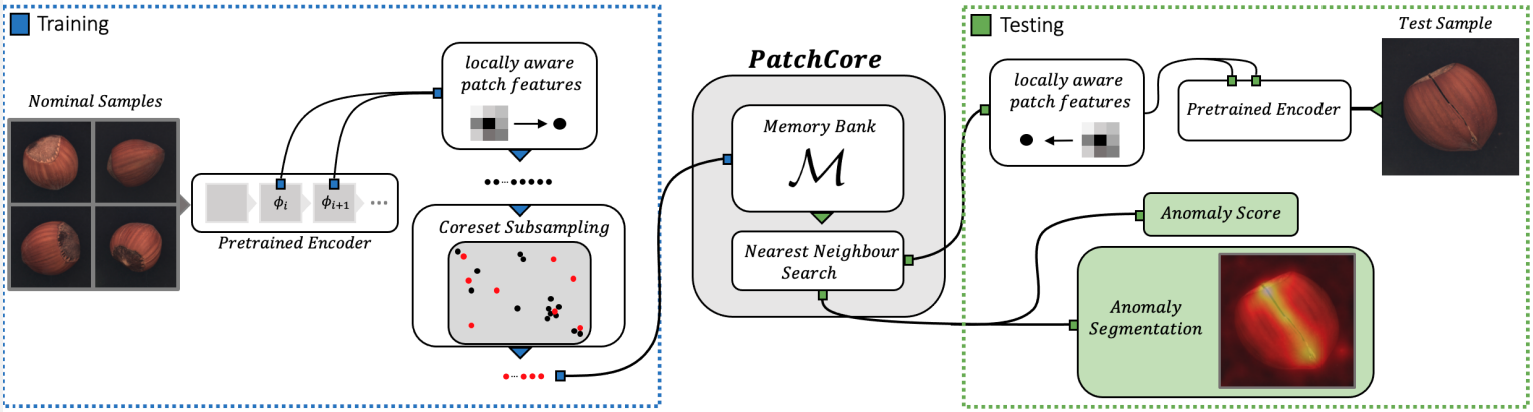
\includegraphics[width=0.95\textwidth]{bilder/patchcore.png}
    \caption{PatchCore}
    \label{fig:PatchCore}
\end{figure}
\subsection{Erzeugen der Patch Features}\label{subsec:ErzeugenDerPatchFeatures}
Zunächst werden einige Notationen definiert, die im Folgenden verwendet werden. Es wird sich dabei auf die Notationen aus der Veröffentlichung bezogen.\
So wird die Menge aller Trainingsbilder als $\mathcal{X}_{train}$ bezeichnet. Die Menge aller Testbilder als $\mathcal{X}_{test}$.\
Für den Trainingsdatensatz gilt im Sinne der Unüberwachtheit, dass es sich um ausschließlich nominale Samples handelt. Im Testdatensatz können sowohl nominale als auch anomale Samples enthalten sein.\
% Werden nominale Samples mit $0$
Bezeichnen wir die wahre Klassenzugehörigkeit eines Bildes $x$ als $y_{x}$, so kann diese entweder $0$ (nominal) oder $1$ (anomal) sein. Für den Trainingsdatensatz gilt dann:\
$\forall x \in \mathcal{X}_{train}: y_{x} = 0$ und für den Testdatensatz $\forall x \in \mathcal{X}_{test}: y_{x} \in \{0,1\}$.\\
Den bereits in \ref{sec:SPADE} und \ref{sec:PaDiM} angetroffenen \glqq Pretrained Encoder\grqq{} wird als $\phi$ bezeichnet.\
Es wird dabei, wie bereits gesehen, nicht der Ausgang dieses Netzwerkes benutzt, sondern die Feature Maps aus einer bestimmten Schicht $j$ des Netzwerkes. \
Im Falle von ResNets, die auch in dieser Veröffentlichung hauptsächlich verwendet werden, ist $j\in \{1,2,3,4\}$.\ 
$j$ wird folgend auch als \glqq Hierarchielevel\grqq{} bezeichnet und spielt eine wichige Rolle.\
$\phi_{i,j} = \phi_{j}(x_{i})$ bezeichnet die Feature Map des Bildes $x_{i}\in \mathcal{X}$ aus dem Hierarchielevel $j$.\
Wie bereits in \ref{subsec:SPADEResults} diskutiert, ist eine sinnvolle Auswahl der Hierarchielevel eine wichtige Voraussetzung für gute Ergebnisse.\
Auch die Autoren von PatchCore weisen auf diese Problemstellung hin. Man könne, wie bei SPADE, die letzte Ebene in der Merkmalshierarchie des Netzes verwenden. \
Dies bringe aber die folgenden zwei Probleme mit sich. Erstens gehe dabei mehr lokalisierte nominale Informationen verloren. Das sei während der Trainingsphase kritisch, \
weil die Arten von Anomalien, die zum Testzeitpunkt auftreten, nicht im Voraus bekannt seien und die möglichst vollständige Erfassung des Normals notwendig sei.\
Zweitens seien die sehr tiefen und abstrakten Merkmale in den vortrainierten ImageNet-Netzwerken auf die Aufgabe der Klassifizierung natürlicher Bilder ausgerichtet, \ 
welche nur wenig direkte Überschneidungen mit der hier vorliegenden Aufgabe der industriellen aufweise. \
Es wird deshalb vorgeschlagen, Merkmale aus den mittleren Hierarchieleveles zu verwenden. Das entspricht bei ResNets $j\in \{2,3\}$.\
Wie in \ref{fig:ResNetPyramid} zu erkennen, handelt es sich bei $\phi_{i,j}$ um einen dreidimensionalen Tensor: $\phi_{i,j}\in \mathbb{R}^{c^{*}\times h^{*}\times w^{*}}$\
mit $c^{*}$ als Tiefe der Feature Maps, $h^{*}$ als Höhe und $w^{*}$ als Breite. \
$\phi_{i,j}(h,w)\in\mathbb{R}^{c^{*}}$ bezeichnet dann den zur Position $h\in\{1,...,h^{*}\}$ und $w\in\{1,...,w^{*}\}$ gehörenden Vektor der Länge $c^{*}$.\
Unter der Annahmen, dass die Größe des Feldes im Originalbild $x_{i}$, das Einfluss auf ein $\phi_{i,j}(h,w)$ nimmt (\glqq Receptive Field\grqq{}), \
ausreichend groß ist, um einen ausreichenden räumlichen Kontext zu erfassen, eignet sich dieser Vektor als \glqq Patch Feature\grqq{} für eine gegenüber \ 
räumlichen Variationen robuste Anomaliedetektion.\\
Um diese wünschenswerte Annahme zu erfüllen, wird eine Aggregation der lokal umliegenden Regionen (\glqq local Neighborhood Aggregation\grqq{}) durchgeführt, das nachfolgend \
vorgestellt wird und die Größe des Receptive Fields steuert.\\
Dafür wird die oben eingeführte Notation für $\phi_{i,j}(h,w)$ um eine ungerade Feldgröße (\glqq patchsize\grqq{}) $p$ erweitert, die die benachbarten Feauture Vektoren \
mit einbezieht. Zunächst wird diese Nachbarschaft wie folgt definiert:\
$$
\mathcal{N}_{p}^{(h,w)} = \{(a,b)| a \in [h-\left\lfloor \frac{p}{2}\right\rfloor,...,h+\left\lfloor \frac{p}{2} \right\rfloor], b \in [w-\left\lfloor \frac{p}{2}\right\rfloor,...,w+\left\lfloor \frac{p}{2}\right\rfloor]\}
$$ 
Damit ergeben sich schließlich die \glqq Patch Features\grqq{} zu\
$$
\phi_{i,j}\Big(\mathcal{N}_{p}^{(h,w)}\Big) = f_{agg}\Big(\{\phi_{i,j}(a,b)| (a,b) \in \mathcal{N}_{p}^{(h,w)}\}\Big),
$$
wobei $f_{agg}$ eine Aggregationsfunktion ist. Die Aggregationsfunktionsfunktion, die in der PatchCore Methode verwendet wird, ist ein adptives \glqq Average Pooling\grqq{}, \
in einer Dimension, die unabhängig von der Länge der Eingangsfeature, immer eine feste Länge $d$ ausgibt.\
%  Hier wird kurz angerissen, was es mit PatchCore auf sich hat. 
% \begin{itemize}
%     \item Popularität, Erscheinungsdatum, Performance, Ersteller, Zitierungen
%     \item Wie funktioniert PatchCore
%     \begin{itemize}
%         \item Training
%         \item Inferenz/Test
%     \end{itemize}
%     \item Implementierung
%     \item Baseline
%     \item Anpassungen
%     \item Fazit
% \end{itemize}
% NUR DER FCK!

\section{Baseline}
\label{sec:Baseline}
Hallo

\section{Adaptionen}
\label{sec:Adaptionen}
Hallo2
      % -*- TeX -*- -*- DE -*-

\chapter{EfficientAD} \label{ch:EfficientAD}
\section{Einleitung} \label{sec:Einleitung}
\textcolor{green}{\textit{Abgeschlossen: 30.10. v1}}\\
Das im Zusammenhang mit dem hier verwendeten Datensatz prominent vertretene Unternehmen MVTec GmbH aus München entwickelte die Methode \textbf{EfficientAD}\ 
und veröffentlichte diese am 25. März 2023. Es handelt sich also um eine junge Methode, die sich \
durch geringe Laufzeiten auf einer GPU und gleichzeitig hoher Genauigkeit auszeichnet. \
Dies ist in \ref{fig:efficientadoverview} dargestellt. Rot markiert sind hierbei die Methoden, die in dieser Arbeit implementiert wurden. \
\begin{figure}[h]
    \centering
    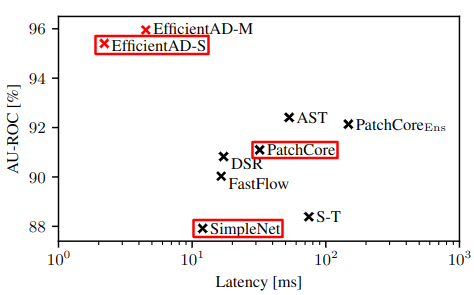
\includegraphics[width=0.4\textwidth]{bilder/overviewspeedauroc.png}
    \caption{Übersicht über AUROC und Laufzeit verschiedener Methoden ausgeführt auf Nvidia RTX A6000 GPU. \cite{efficientad}}
    \label{fig:efficientadoverview}
\end{figure}
Mit bis zu \num{99,8}\% Instanzklassifiziergungsgenauigkeit auf dem Datensatz MvTecAD ist es die Methode mit der höchsten\
Genauigkeit auf diesem Datensatz. \cite{paperswithcode}\\
Es kombiniert dabei verschiedene Methoden, die in anderen Veröffentlichungen schon erfolgreich eingesetzt wurden.\
So wird ein zweiteiliger \glqq Student-Teacher\grqq{}-Ansatz verwendet.\
Zum einen erkennen wir eine modifizierte Variante der Exktraktion von Featuren durch ein auf ImageNet implizit vortrainiertem Netz\
(Wissens-Distillation). Der andere Teil setzt auf einen Student-Teacher-Ansatz auf Basis eines Autoencoder, der die Aufgabe hat, nominale Merkmale\
zu rekonstruieren. Beide Konzepte werden in diesem Kapitel noch genauer erläutert.\\
Die Implementierung erfolgt dabei beinahe ausschließlich mithilfe von CNNs. Nur die finale Bestimmung des Anomalie-Scores und der Anomaliekarte,\
die, wie gezeigt werden wird, kaum laufzeitkritisch ist, wird ohne die Verwendung von CNNs realisiert.\
Da moderne GPUs äußerst schnelle Inferenz von CNNs ermöglichen, gehört diese Methode zu den am schnellsten ausführbaren Methoden im Bereich\
der Unüberwachten Anomaliedetekion.\cite{efficientad}\cite{paperswithcode} \\
Wie bereits gesehen werden konnte, lassen sich solche Aussagen über die Laufzeit nicht einfach übertragen, liegt keine GPU vor, wie in\
dieser Arbeit.\\
\section{Grundlage - Uninformed Students}\label{sec:GrundlageUninformedStudents}
\textcolor{green}{\textit{Abgeschlossen: 02.11. v1}}\\
Die Veröffentlichung \glqq Uninformed Students: Student-Teacher Anomaly Detection with Discriminative Latent Embeddings\grqq{}, welche am 18. März 2020\
vorgestellt wurde, präsentiert ein zentrales Konzept, welches auch in EfficientAD verwendet wird.\
Die ebenfalls von MVTec GmbH entwickelte Methode setzt somit auch auf eine Student-Teacher-Architektur.\
\subsection{Funktionsweise}
In diesem Bereich wird genauer auf die Funktionsweise von \glqq Uninformed Students\grqq{} eingegangen.\
Analog zu den bisher beschriebenen Methoden, wird zunächst der aus nominalen Bilder bestehende Trainingsdatensatz als
$\mathcal{X}_{train}={x_1, x_2, ..., x_n}$ ($\forall x \in \mathcal{X}_{train}: y_{x}=0$) definiert.\
Das Ziel ist es, ein Ensemble an \glqq Studenten\grqq{} $S_{i}$ zu erzuegen, die später in der Lage sind, Anomalien \
eines anomalen Testbildes $x_{i}\in\mathcal{X}_{test}$ und $y_{x} = 1$ mit $\forall x \in \mathcal{X}_{test}: y_{x}=\{0,1\}$ zu erkennen.\
Um eine solche Aussage zu treffen, wird die Abweichung für ein Testbild $x_{i}$ von der Ausgabe der Studenten $S_{i}$\
und der des \glqq Lehrers\grqq{} (Teacher) $T$ bestimmt. Große Abweichungen deuten dabei auf eine Anomalie hin.\
Der Teacher $T$ ist dabei ein CNN, welches auf einem großen Datensatz, wie ImageNet, vortrainiert wurde.\
Es kommen dabei keine ResNets diekt zum Einsatz, sondern einfache CNNs, die von den Autoren selbst entwickelt wurden.\
Die Architektur von Teacher $T$ und Studenten $S_{i}$ ist dabei identisch.\
\subsubsection*{Lernen von lokalen Patch Deskriptoren}
In diesem Abschnitt wird sich damit beschäftigt, wie ein Teacher $T$ in die Lage versetzt wird,
deskriptive und lokal aufgelöste Merkmale zu extrahieren. %Die Techniken, die dazu verwendet werden sind \
%\textbf{Wissens-Distillation} und \textbf{Metric-Learning}.\
$\hat{T}$ kann für beliebige $p\in\mathbb{N}$ aus einem Bild oder Bildausschnitt $\mathbf{p}\in\mathbb{R}^{p\times p\times C}$ einen eindimensionalen Feature Vektor\
erzeugen.\ 
Drei verschiedene Wege des Lernens des Teachers werden im Folgenden beschrieben.\
\paragraph*{Wissens-Distillation}\label{par:wissensdistillation}
Wie bereits ausführlich in \ref{subsec:ResNetsAsFeatureExtractor} und in den vorangegangenen Methoden beschrieben,\
dienen CNNs, die auf großen Datensätzen vortrainiert wurden, als Feature-Extraktoren für aussagekräftige und kompakte Merkmalsextraktoren.\
Um ein leichtgewichteren Featre Extraktor zu erhalten, wird das CNN $\hat{T}$ trainiert um das Verhalten eines großen, auf ImageNet vortrainierten\
CNNs $\phi$ zu imitieren. Es werden dazu Bilder aus ImageNet auf die Größe $p\times p$ ausgeschnitten und dienen als Eingangsgröße.\
Das Label könnte nun direkt aus einem Einbettungsprozess wie bei \ref{subsec:ErzeugenDerPatchFeatures} erzeugt werden, es ergeben sich\
aber Probleme durch unterschiedliche Größen der jeweiligen Ausgaben. Deshalb wird zusätzliche ein einfaches vollvernetztes neuronales Netz (MLP)\
eingesetzt, dass die Ausgaben des Netzwerkes $\phi$ auf die gewünschte Größe $d$ abbildet.\
Folgende Verlustfunktion wird verwendet, um das Netzwerk $T$ zu trainieren:\
$$
\mathcal{L}_{KD} = \left\lVert D(\hat{T}(\mathbf{p}))-\phi(\mathbf{p}) \right\rVert_{2}^{2}
$$
$\hat{T}$ ist jedoch auf eine Eingabe von $p\times p$ Pixeln beschränkt, soll ein eindimensionaler Feature Vektor erzeugt werden. \
Das Netzwerk $\hat{T}$ muss dementsprechend noch in die Lage versetzt werden, mit größeren Bildern umzugehen. Die Autoren dieser Veröffentlichung \
gehen dabei nach \cite{bailer2018fast} vor und erhalten so einen effizienten Feature Extraktor $T$.\
Für $\hat{T}$ werden drei verschiedene Architekturen verwendet, die sich in ihrer Komplexität und der Größe des rezeptiven Feldes ($p\in\{17,33,65\}$) unterscheiden. \
Für weitere Details wird an dieser Stelle auf die Veröffentlichung \cite{bailer2018fast} verwiesen, weil es hier vor allem um das Konzept \
und dessen Erläuterung gehen soll.\\
Das für die Wissens-Distillation verwendete Netzwerk $\phi$ ist ein ResNet-18, welches auf ImageNet vortrainiert wurde. Es wird dabei der 1D-Feature-Vektor \
aus der letzten Schicht des ResNets (\glqq flatten\grqq{} in \ref{fig:ResNetPyramid}) verwendet. Dieser 512 Einträge fassender 1D-Vektor wird mithilfe von $D$ auf $d=128$\
Einträge komprimiert. Es sei angemerkt, dass es sich hierbei um die Werte aus der Originalveröffentlichung handelt und andere Wertekombinationen ebenfalls möglich sind. \
\paragraph*{Metrisches Lernen}\label{par:metrischeslernen}
Beim metrischen Lernen wird zunächst ein Triplet aus Patches $(\mathbf{p}, \mathbf{p}^{+}, \mathbf{p}^{-})$ erzeugt. Das Ausgangspatch $\mathbf{p}$\
wird dabei durch einen zufällig ausgeschnittenen Bildausschnitt aus einem Bild aus dem Trainingsdatensatz erzeugt.\
$\mathbf{p}^{+}$ ist eine mit Gauß'schen Rauschen und veränderte Helligkeit augmentierte Version von $\mathbf{p}$.\
Bei $\mathbf{p}^{-}$ handelt es sich um einen Bildausschnitt aus einem anderen Bild aus dem Trainingsdatensatz.\
Die Verlustfunktion für das metrische Lernen ist dann gegeben durch: \
$$
\mathcal{L}_{M} = \max\left\{0,  \delta + \delta^{+}-\delta^{-}\right\}
$$
$$
\delta^{+}=\left\lVert \hat{T}(\mathbf{p})-\hat{T}(\mathbf{p}^{+}) \right\rVert_{2}^{2}
$$
$$
\delta^{-}=\min\left\{\left\lVert \hat{T}(\mathbf{p})-\hat{T}(\mathbf{p}^{-}) \right\rVert_{2}^{2}, \left\lVert \hat{T}(\mathbf{p}^{+})-\hat{T}(\mathbf{p}^{-}) \right\rVert_{2}^{2} \right\}
$$
Dabei bezeichnet $\delta>0$ einen Randparameter, der einen Hyperparameter bzgl. des Trainings darstellt. \
Minimiert man diese Verlustfunktion, so wird das Netzwerk $\hat{T}$ in die Lage versetzt, ähnliche Patches in einem Feature Raum nahe beieinander zu platzieren und die distinkten\
Patches weiter voneinander zu entfernen. Es wird also die diskriminative Fähigkeit des Netzwerkes $\hat{T}$ gestärkt.\
\paragraph*{Kompaktheit der Merkmale}\label{par:kompaktheitdermerkmale}
Um eine kompakte und möglichst wenige redundante Representation der Merkmale zu erhalten, wird ein weitere Verlustfunktion eingeführt. \
$$
\mathcal{L}_{C}\left(\hat{T}\right) = \sum_{i\neq j} c_{ij} 
$$
Die skalaren Parameter $c_{ij}$ bezeichnen dabei die Einträge der Korrelationsmatrix über alle $\hat{T}\left(\mathbf{p}\right)$ für sämtliche $\mathbf{p}$ im aktuellen Mini-Batch des \
Trainings. Indem die Einträge auf der Diagonalen nicht minimiert werden, die Einträge außerhalb der Diagonalen jedoch schon, wird eine Darstellung gefördert, \
die die einzelnen Merkmale, welche $d$-fach im Feature Vektor gebündelt sind, entkoppelt, also unabhängig voneinander macht. \\
Die finale Verlustfunktion ergibt sich dann aus einer Linearkombination dieser drei Verlustfunktionen: \
$$
\mathcal{L}_{T} = \lambda_{KD}\mathcal{L}_{KD} + \lambda_{M}\mathcal{L}_{M} + \lambda_{C}\mathcal{L}_{C}, \quad \lambda_{KD}, \lambda_{M}, \lambda_{C} \in \mathbb{R}^{+}
$$
Die Faktoren $\lambda_{KD}, \lambda_{M}, \lambda_{C}$ sind dabei Hyperparameter, die das Training beeinflussen. \
\subsubsection*{Lernen der Studenten}
Nun wird sich mit dem Training der Studenten $S_{i}$ beschäftigt. Diese sollen in die Lage versetzt werden, \
nominale Patches in der selben Weise, wie der Teacher $T$ zu extrahieren, also dessen Ausgabe auf nominalen Bildern zu imitieren.\
Liegt ein anomales Bild vor, so soll die Ausgabe der Studenten möglichst stark von der des Teachers abweichen.\\
Zunächst wird die Ausgabe des trainierten Teachers $T$ über alle Bilder in $\mathcal{X}_{train}$ erzeugt. Aus den so entstandenen Merkmalsvektoren wird dann\
der Mittelwert $\boldsymbol{\mu}\in\mathbb{R}^{d}$ und die Standardabweichung $\mathbf{\sigma}\in\mathbb{R}^{d}$ komponentenweise bestimmt.\
Für jede mögliche Position $(h,w)$ mit $h\in\{1,...,h^{*}\}$ und $w\in\{1,...,w^{*}\}$ wird dann die Ausgabe $y$ der Studenten $S_{i}$ bestimmt\
und als Gaußverteilung $P\left(\mathbf{y}|\mathbf{p}_{h,w}\right)=\mathcal{N}\left(\mathbf{y}|\boldsymbol{\mu}^{S_{i}}_{h,w},s\right)$ mit konstanter\ 
Kovarianz $s\in\mathbb{R}$ modeliert. $\boldsymbol{\mu}^{S_{i}}_{h,w}$ ist hierbei die Prädiktion von $S_{i}$ zur Stelle $\left(h,w\right)$.\
Sei nun $\mathbf{y}^{T}_{h,w}$ die von den Studenten zu prädizierende Zielgröße, also die Ausgabe des trainierten Teachers, ergibt sich damit folgende\
Verlustfunktion für das Training des Studenten:\\
$$
\mathcal{L}\left(S_{i}\right)= \frac{1}{h^{*}w^{*}} \sum_{\left(h,w\right)\in \left\{1,...,h^{*}\right\} \times \left\{1,...,w^{*}\right\}} \left\lVert \boldsymbol{\mu}^{S_{i}}_{h,w} - \left(\mathbf{y}_{h,w}^{T}-\boldsymbol{\mu}\right)diag\left(\boldsymbol{\sigma}^{-1}\right) \right\rVert_{2}^{2}
$$
$diag\left(\boldsymbol{\sigma}\right)^{-1}$ ist dabei die Inverse der Diagonalen der Matrix, die mit den Werten aus $\boldsymbol{\sigma}$ gefüllt ist.\
\subsubsection*{Bestimmen des Anomaliegrades}\label{subsubsec:bestimmendesanomaliegradesUninformedStudents}
Nach dem Training der Studenten bis zur Konvergenz, wird für jeden Position $(h,w)$ eines Bildes eine Gauß-Mixtur bestimmt. Dies geschieht über alle Studenten des Ensembles, die alle gleichgewichtet eingehen. \
Damit kann auf zwei verschiedene Wege ein Anomaliegrad bestimmt werden. \\
Zunächst lässt sich der Regressionsfehler zwischen der Ausgabe des Teachers und dem Mittelwert der Ausgaben der Studenten bestimmen. \
$$
e_{h,w} = \left\lVert \boldsymbol{\mu}_{h,w} - \left(\mathbf{y}_{h,w}^{T}-\boldsymbol{\mu}\right)diag\left(\boldsymbol{\sigma}^{-1}\right) \right\rVert_{2}^{2} 
$$
$\boldsymbol{\mu}_{h,w}$ ist hierbei der Mittelwert der Ausgaben der Studenten an der Position $(h,w)$ ($\boldsymbol{\mu}_{h,w}=\frac{1}{M} \sum_{i=1}^M\boldsymbol{\mu}_{h,w}^{S_i}$). \
Die Idee ist nun, dass ein hoher Regressionsfehler auf eine Anomalie hinweist, weil die Studenten nicht in der Lage sind, \
die Ausgabe des Teachers zu imitieren. \\
Eine andere Möglichkeit der Bestimmung eines Anomaliegrades ist es, die Unsicherheit der Prädiktionen der Studenten zu betrachten.\
Dies basiert auf der Annahme, dass die Augaben der Studenten auf nominalen Bildern eine geringere Varianz aufweisen, als auf anomalen Bildern, weil\
diese Ungesehenes beinhalten, für das das jeder Student $S_{i}$ eine andere, zufällig streuende Prädiktion ausgibt.\
Quantitativ kann das wie folgt formuliert werden:\
$$
v_{h,w}=\frac{1}{M} \sum_{i=1}^M\left\|\boldsymbol{\mu}_{h,w}^{S_i}\right\|_2^2-\left\|\boldsymbol{\mu}_{h,w}\right\|_2^2
$$
Mit einer Normalisierung der jeweiligen Größen $e_{h,w}$ und $v_{h,w}$ mithilfe der Mittelwerte und Standardabweichung über alle Positionen $(h,w)$ folgt \
schließlich das für ein Studeten-Teacher-Paar finale Anomaliemaß für die Position $(h,w)$: \
$$
\tilde{s}_{h,w}=\tilde{e}_{h,w}+\tilde{v}_{h,w}=\frac{e_{h,w}-e_\mu}{e_\sigma}+\frac{v_{h,w}-v_\mu}{v_\sigma} .
$$
Weitergehend kann nur ein Ensemble an Student-Teacher-Paaren verwendet werden, um die Anomalieklassifikation zu verbessern. \
Sinnvoll ist es, solche Paare zu trainieren, die unterschiedliche rezeptive Felder $p$ aufweisen. Dann können Anoamlien unterschiedlicher Größe \
detektiert werden, ohne dass ein Hoch oder Runterskalieren des Bildes notwendig ist, was immer mit einem Informationsverlust einhergeht. \
Für $L$ Student-Teacher-Paare ergibt und die die jeweiligen Anomliegrade $\tilde{s}_{h,w}^{(l)}$, ergibt sich dann \
$$
s_{h,w}=\frac{1}{L}\sum_{l=1}^L\tilde{s}_{h,w}^{(l)} .
$$
\subsection{Ergebnisse und Diskussion}
Es handelt sich bei dieser Methode um die älteste in dieser Arbeit beschriebene Methode.\
Viele Erkentnisse, die in den darauffolgenden Jahren durch zahlreiche Veröffentlichungen gewonnen wurden, fehlten\
den Autoren dieser Veröffentlichung. So wurde als Lernziel für den Teacher $T$ und die Wissensdistillation ein ResNet 18 verwendet, dessen Feature dann mittels PCA in die richtige Dimension gebracht wurde.\
Heute ist bekannt, dass tiefere Netze bessere Feature Extraktoren sind und PCA keine geeignete Methode ist, um Patch Feature zu reduzieren. Letzteres wurde z.B. in PaDiM festgestellt, aber auch in qualitativen Untersuchungen in dieser Arbeit.\
Auch das metrische Lernen erweist sich als nicht hilfreich, wie bereits die Autoren selbst in ihrer Veröffentlichung feststellen.\\
Vor diesem Hintergrund ist die erzielte Genauigkeit dennoch beachtlich und entspricht in etwa den Ergebnissen von SPADE. Der Fokus in dieser Arbeit lag nicht auf einer\
Instanzklassifiziergung, sondern auf der Segmentierung, weswegen hierfür weder eine Methode, noch Ergebnisse veröffentlicht wurden. Aufgrund der pixelweisen Metriken, die in der Veröffentlichung angeben sind und an dieser Stelle\
nicht weiter besprochen werden, lässt sich diese Aussage treffen.\\
Auch Aussagen zur Laufzeit müssen qualitativ erfolgen. Es ist nicht davon auszugehen, dass durch die Vielzahl an Elementen ($M=3$ und $L=3$) die Laufzeit geringer ist, als bei den anderen Methoden.\
Insgesamt müssten bei einem solchen Konfiguration, wie sie in der Veröffentlichung angegeben ist, 9 CNNs auf einem Bild ausgeführt werden.\\
Viel wichtiger als die tatsächlichen Ergebnisse, sind aber die Impulse, die durch diese Arbeit gesetzt wurden. Folgende Erkentnisse sind hierbei besonders hervorzuheben:\
\begin{itemize}
    \item Eine Feature Exktrattion durch Wissensdistillation ist möglich und ermöglicht spezifisch angepasste Feature Extraktoren, die auf die Aufgabe zugeschnitten sind.\
    \item Ein Student-Teacher Ansatz ist eine geeignete Methode, um Anomalien zu detektieren.\
    \item Verschieden aufgelöste Feature Maps können zu einer Verbesserung der Anomaliedetektion führen.\
\end{itemize}
In nachfolgendem Abschnitt zur Funktionsweise von EfficientAD werden einige dieser Erkentnisse aufgegriffen und weiterentwickelt.\
\section{Funktionsweise von EfficientAD}\label{sec:funktionsweisevonEfficientAD}
\textcolor{green}{\textit{Abgeschlossen: 02.11. v1}}\\
In diesem Abschnitt wird die Funktionsweise der Methode EfficientAD beschrieben. Es wird hauptsächlich das Konzept des \
Student-Teacher Designs, das in \ref{sec:GrundlageUninformedStudents} beschrieben wurde, verwendet. \
Dabei gibt es zwei, konzeptionell unterschiedliche Student-Teacher Paare, die jeweils unterschiedliche Aufgaben erfüllen. \
\subsection{Feature Extraktion}\label{subsubsec:featureextraktionEfficientad}
Ein wesentlicher Unterschied zu PatchCore und SimpleNet ist, dass für die Feature Exktration \
nicht auf explizit auf ein vortrainiertes ResNet gesetzt wird. \ 
Zwar wird diese Grundidee immer noch beibehalten, insofern, als dass ein solches ResNet verwendet wird, \
um den eigentlichen Feature Extraktor zu trainieren. Während der Inferenz wird jedoch kein ResNet verwendet. \
Stattdessen kommt ein sogenannter \textbf{Patch Description Network (PDN)} zum Einsatz, welches mithilfe von Wissens-Distillation \ 
trainiert wird. Es besteht aus lediglich vier Convolutional-Layern, die in \ref{fig:pdn} dargestellt sind.\\
\begin{figure}[h]
    \centering
    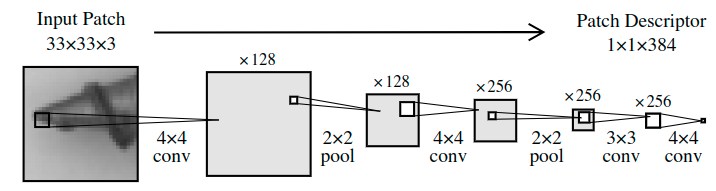
\includegraphics[width=0.8\textwidth]{bilder/pdn.png}
    \caption{Skizze der Architektur des Patch Description Networks (PDN). \cite{efficientad}}
    \label{fig:pdn}
\end{figure}
In \ref{fig:pdn} zu sehen, ist, dass die Ausgabe eines PDN 384-dimensionale Feature-Vektoren sind, deren rezeptives Feld exakt $p=33$ Pixel beträgt.\
Dies entspricht der Idee, die bereits drei Jahre zuvor in \glqq Uninformed Students\grqq{} \cite{uninformedstudents} vorgestellt wurde.\
Im Falle eines ResNets als Feature Exktraktor kann das rezeptive Feld selten grenzscharf bestimmt werden, wodurch sich das PDN für Segmentierungsaufgaben\
in dieser Hinsicht besser eignet. \\
Eine räumliche Dimensionsreduktion findet durch ein schrittweises Average-Pooling nach den ersten beiden Convolutional-Layers statt. Die geringere Dimension der\
Feature Maps sorgen für eine schnellere Laufzeit. Wie noch zu sehen sein wird, ist diese Dimensionsreduktion allerdings deutlich zurückhaltender, als zum Beispiel bei ResNet-Architekturen.\\
Durch den vollständig aus Convolutional- und Pooling-Layern bestehende Aufbau des PDN, ist es möglich, alle Feature Vektoren eines Bildes in einem\
Durchlauf zu extrahieren.\
Es stehen zwei verschiende PDNs zur Verfügung, welche sich in ihrere Größe und daraus resultierend, ihrer Laufzeit unterscheiden.\
Insbesondere die Anzahl an Filter in den Convolutional-Layern unterscheidet sich, also die Anzahl an Channels. Diese ist im Falle des größeren Netzes \
deutlich höher. Für Details hierzu wird auf die Veröffentlichung \cite{efficientad} und Tabelle 5 bzw. 6 verwiesen.\\
Wie bereits erwähnt, erfolgt das Training des PDNs mithilfe von Wissens-Distillation von einem vortrainierten ResNet.\
In \ref{par:wissensdistillation} wurde bereits beschrieben, wie ein solcher Distillationsprozess aussieht.\
Definieren wir den PDN als $T:\mathbb{R}^{3\times 256\times 256}\rightarrow \mathbb{R}^{384\times 64\times 64}$ benötigen wir einen vortrainierten \
Feature Extraktor $\phi:\mathbb{R}^{3\times W\times H}\rightarrow \mathbb{R}^{384 \times 64\times 64}$, der auf ImageNet vortrainiert wurde. \
Die Kantenlängen $W$ und $H$ sind dabei so zu wählen, dass die Ausgabe des Feature Extraktors $\phi$ $64\times 64$ Pixel groß ist.\
Hierzu eignet sich ein Feature Extraktor, wie in \ref{subsec:ErzeugenDerPatchFeatures} bei der Methode PatchCore verwendet, ideal.\
Es wird auch in der Veröffentlichung der Einbettungsprozess aus \ref{subsec:ErzeugenDerPatchFeatures} verwendet und ein Wide ResNet 101 \cite{wideresnet}.\
Die Verlustfunktion für das Training des PDNs auf mit einem Bild $x\in\mathcal{X}_{train}$ ergibt sich dann einfach zu:\
$$
\mathcal{L}= \left\lVert T(x)-\phi(x) \right\rVert_{2}^{2}
$$
$\mathcal{X}_{train}$ ist hierbei aus dem ImageNet Datensatz entnommen. Es handelt sich also um einen $L2$-Loss. \ 
Die Auflösung $H \times W$ der Bilder aus ImageNet beträgt in diesem Fall, also mit einem Wide ResNet 101, $512\times 512$ Pixel. \\
\subsection{Reduzierter Student-Teacher Ansatz}
Die in \ref{sec:GrundlageUninformedStudents} beschriebene Methode \glqq Uninformed Students\grqq{} wird in EfficientAD in einer reduzierten Form verwendet.\
Es wird kein Ensemble an Studenten verwendet, sondern nur ein einzelner Student, was $M=1$ in \ref{subsubsec:bestimmendesanomaliegradesUninformedStudents} entspricht.\
Ebenfalls kommt lediglich eine Student-Teacher Paarung in diesem Schritt zum Einsatz. Gegenüber der Veröffentlichung \glqq Uninformed Students\grqq{}\cite{uninformedstudents}\ 
ist das eine weitere Vereinfachung. Diese dienen in erster Linie einer kürzeren Laufzeit.\\
Der Teacher $T$ ist dabei durch das PDN, trainiert durch Wissensdistillation, gegeben. Für den Studenten $S$ wird die Architektur identisch übernommen.\\
Es wird somit auch auf eine asymetrische Architektur verzichtet, wie sie erfolgreich in \cite{ast} angewandt wurde.\
Stattdessen wird auf eine angepasste Verlustfunktion zurrückgegriffen, die im Folgenden beschrieben wird.\\
Grundsätzlich besteht die Schwierigkeit beim Trainieren eines Student-Teacher Paares darin, den Studenten zwar soweit zu trainieren, dass er in der Lage ist,\
das Verhalten des Teachers auf nominalen Beispielen möglichst genau zu imitieren, aber dennoch nicht genug generalisiert zu haben, dies auch in einem anomalen Fall zu tun.\
Es entsteht ein Trade-Off, der in dieser Veröffentlichung clever gelöst wird.\\
So wird zunächst ein Verfahren eingeführt, dass nur Bereiche im Bild für das Anpassen der Parameter mithilfe von Backpropagation verwendet, welche \
besonders große Abweichungen zwischen der Ausgabe des Teachers und des Studenten aufweisen. Geringfügige Abweichungen werden ignoriert.\\
Formal wird dazu ein Trainingsbild $x \in \mathcal{X}_{train}$ verwendet, um die Ausgabe sowohl des Studenten $S(x)$, als auch des Teachers $T(x)$ zu bestimmen.\
Dabei ist $T(x), S(x) \in \mathbb{R}^{C \times H \times W}$. Daraus wird dann die quadratische Differenz $D_{c,w,h} = \left(T(x)_{c,w,h}-(S(x)_{c,w,h})\right)^{2}$\
für jedes Element $(c,h,w)$ bestimmt. Der Idee folgend, nur die größten Differenzen eingehen zu lassen, wird anschließend ein Schwellwert $d_{hart}$ berechnet,\
der von einem Hyperparameter $p_{hart} \in \left[0,1\right]$ abhängt. Dieser bestimmt, wie groß die Menge an Elementen aus $D_{c,w,h}$ ist, die für das Training verwendet werden.\
Es gilt, dass $d_{hart}$-Quantil $d_{hart}$ ist. Für $p_{hart}=\num{0,999}$ werden laut \cite{efficientad} etwa 10\% der Elemente aus $D_{c,w,h}$ für das Training verwendet.\
Würde $p_{hart}=0$ gewählt, so würden alle Elemente $D_{c,w,h}$ für das Training verwendet. \ Konkret wird dann die Verlustfunktion $\mathcal{L}_{hart}$ zum Durchschnitt\
über alle Werte aus $D$ bestimmt, für die gilt, dass $D_{c,w,h} \geq d_{hart}$.\\
In der Praxis führt dieser Ansatz dazu, dass nur wesentliche Bereiche im Bild für das Training verwendet werden. Veranschaulicht ist das in nachfolgender Abbildung, welche der\
Veröffentlichung entnommen wurde (\ref{fig:hardthreshold}). Es ist zu erkennen, dass Objektbereiche in $\mathcal{L}_{hart}$ eingehen, der Hintergrund hingegen bereits vom Studenten\
gut imitiert wird und somit nicht mehr in die Verlustfunktion eingeht.\\
\begin{figure}[h]
    \centering
    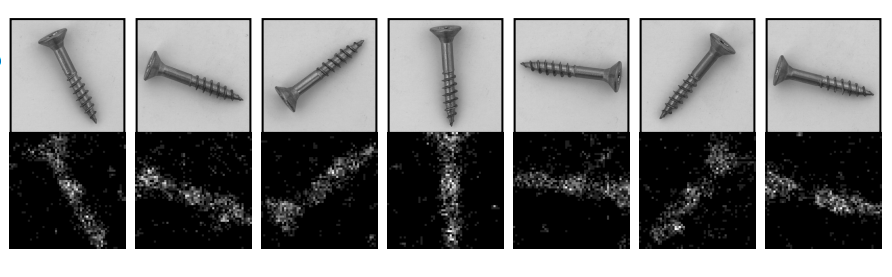
\includegraphics[width=0.8\textwidth]{bilder/hardloss.png}
    \caption{Veranschaulichung der \glqq Hard Loss\grqq{}-Filterung für $\mathcal{L}_{hart}$. Obere Reihe stellt Trainingsbilder dar, Untere die Masken. Alle dunklen Bereiche werden ignoriert, helle Bereiche werden zum Training verwendet. \cite{efficientad}}
    \label{fig:hardthreshold}
\end{figure}
Zusätzlich zu dieser speziellen Verlustfunktion, die für das Training des Studenten verwendet wird, wird ein Strafterm eingeführt, der den Studenten daran hindert,\
den Teacher auf Bildern, die nicht Teil der nominalen Trainingsdaten sind, zu imitieren.\ 
In einem klassischen Setup würde der Student vom Teacher nur mit Bildern lernen, die nominal und aus der Zieldomäne stammend sind. Der Teacher hingegen würde auf einem größeren,\ 
breter gefassten Datensatz trainiert werden, zum Beispiel mit ImageNet.\ 
In dieser Veröffentlichung wird der Student zusätzlich auf Bildern trainiert, die aus dem ImageNet Datensatz stammen.\
Konkret wird in jedem Trainingsschritt ein Bild $x_{imagenet}$ aus ImageNet zufällig ausgewählt und mit der Verlustfunktion $\mathcal{L}_{Strafterm}=\frac{\sum_{c}\lVert S(x_{imagenet})_{c} \rVert^{2}_{F}}{HWC}$\ 
ein Strafterm bestimmt. Es wird hierfür die Frobenius-Norm über alle Kanäle verwendet. Dieser Strafterm verhindert, dass der Student auf Bildern, die nicht aus der Zieldomäne stammen,\
generalisiert.\\
Die finale Verlustfunktion für den Studenten ergibt sich dann zu:\
$$
\mathcal{L}_{Student}= \mathcal{L}_{hart} + \mathcal{L}_{Strafterm} %TODO --> besseren Namen für "hart"
$$
Eine detailierte Aufschlüsslung des gesamten Trainingsprozesses ist in \cite{efficientad} im Appendix A.1 und Algorithus 1 zu finden.\\
\subsection{Erkennen logischer Anomalien}\label{subsec:erkennenlogischeranomalien}
Wie bereits in der Einleitung zu diesem Kapitel erwähnt, ist EfficientAD in der Lage, neben strukturellen Anomalien, auch logische Anomalien zu erkennen.\
Weil bei PatchCore und SimpleNet keine globale Strukturinformationen verwendet werden, sondern immer nur bereichsweise analysiert wird, ist es nur sehr eingeschränkt möglich\
mit diesen Methoden logische Anomalien zu erkennen. In \ref{sec:DatensatzMVTecAD} wurde bereits erwähnt, dass der MVTec AD Datensatz im Wesentlichen keine logischen Anomalien enthält\
und die Zielsetzung dieser Arbeit nicht die Erkennung logischer Anomalien ist. Deshalb wird diese interessante Fähigkeit von EfficientAD hier nicht weiter betrachtet.\
Auf dem Datensatz MVTec LOCO AD, der ebenfalls in \ref{sec:DatensatzMVTecAD} Erwähnung findet und hautpsächlich logische Anomalien enthält, ist die Methode EfficientAD\
die beste bislang veröffentlichte Methode (Stand Oktober 2023). \cite{mvtecadloco} \\
Um solche Anomalien zu erkennen, wird ein Autoencoder verwendet, um die logischen Zusammenhänge nominaler Bilder zu erlernen. Es wird sich dabei vor allem an der Methode \glqq GCAD\grqq{} \
orientiert \cite{gcad}, die sich mit dem Erkennen logischer Anomalien mithilfe von Autoencodern beschäftigt. Weil dies nicht Schwerpunkt dieser Arbeit ist, wird auf eine Erläuterung \
der Methode GCAD hier verzichtet. Die wesentlichen Aspekte von GCAD finden sich ohnehin in dem hier Beschriebenen wieder.\\
Ebenfalls wird ein Student-Teacher Paar gebildet. Auch hier wird der Student $A$, der durch den Autoencoder implementiert wird, trainiert, um die Ausgabe des Teachers $T$ zu imitieren. \
Formal ergibt sich die Verlustfunktion für das Training des Autoencoders für ein Bild $x$ zu: \
$$
\mathcal{L}_{AE} = \frac{\sum_{c}\left\lVert A(x)_{c}-T(x)_{c} \right\rVert_{F}^{2}}{HWC}
$$
Auch hier ist $T(x), A(x) \in \mathbb{R}^{C \times H \times W}$ und die Frobenius-Norm wird über alle Kanäle verwendet. Das Bild $x$ ist dabei ein Bild aus dem Trainingsdatensatz, der in \
diesem Fall ausschließlich aus nominalen Bildern der Zieldomäne besteht.\\
Im Gegensatz zu den PDNs, die immer nur ein endlich großes rezeptives Feld haben, welches im Falle der PDNs sogar exakt definiert ist, wird vom Autoencoder das gesamte Bild betrachtet.\
Es muss möglichst viel der Bildinformation durch ein \glqq Bottleneck\grqq{} (dt.: Flaschenhals) bringen, um eine Rekonstruktion des Bildes zu ermöglichen. Dieses Bottleneck ist\
dabei lediglich 64 Kanäle fassend, wodurch eine Komprimierung erzwungen wird.\\
Man spricht Im Zuammenhang mit Autoencodern vom Encoder, der die Bildinformation auf einen niedrigdimensionalen Vektor, das Bottleneck, abbildet und dem Decoder, der diesen Vektor wieder\
auf eine größere Dimension abbildet. Diese Zieldimension entspricht dabei nicht der Auflösung des Eingangsbildes, sondern der Auflösung der Patch Feature Vektoren.\\
Auf Bildern mit logischen Anomalien ist die grundsätzliche Struktur des Bildes verschieden zur nominalen Struktur. Da der Autoencoder jedoch aus dem Training nur\
nominale Bilder zu sehen bekommt und diese grundsätzliche Struktur implizit zur möglichst fehlerfreien Rekonstruktion erlernt und ausgenutzt hat, wird der\
Autoencoder nicht in der Lage sein, eine Abweichung der nominalen Struktur ebenfalls korrekt zu rekonstruieren.\\
Autoencoder haben im Allgemeinen die Schwäche, dass die Rekonstruktionen von fein aufgelösten Bilddetails nicht gut gelingt. Dies ist auch hier der Fall.\
Um falsche Positive, also scheinbare Anomalien, die durch eine schlechte Rekonstruktion solcher feiner Strukturen entstehen würden, zu vermeiden, wird die Anzahl der\
Ausgangskanäle des Studenten $S$ verdoppelt und trainiert, die Ausgabe des Autoencoders zu imitieren.\
Definiert man nun den Teil des Studenten, der mit dem Autoencoder korrespondert mit $S^{\prime}$ und $S^{\prime}(x) \in \mathbb{R}^{C \times H \times W}$ als die Ausgabe\
dieses Teils des Studenten, ergibt sich die Verlustfunktion für das Training des Studenten $S^{\prime}$ zu:\
$$
\mathcal{L}_{AE} = \frac{\sum_{c}\left\lVert S^{\prime}(x)_{c}-A(x)_{c} \right\rVert_{F}^{2}}{HWC}
$$
Somit lernt der Student $S^{\prime}$, die systematischen Rekonstruktionsfehler des Autoencoders $A$ mit, wodruch diese nicht mehr zu falschen Positiven führen.\
Außerdem ist der Student $S^{\prime}$ Teil des PDNs, welches ein rezeptives Feld von $p=33$ Pixeln hat. Es ist also nicht in der Lage größere Strukturen zu erkennen und\
somit in aller Regel nicht beeinfluss von logischen Anoamlien.\\
\subsection{Bestimmen des Anomaliegrades}\label{subsec:efficientadbestimmenanomaliegrades}
In beiden oben genannten Paaren, also Autoencoder $A$ und Student $S^{\prime}$ sowie PDN $T$ und Student $S$, kann die Differenz der Ausgaben als Anomaliemaß verwendet werden.\
Konkret wird die pixelweise quadratische Differenz der Ausgaben berechnet.\
Es entstehen somit zwei Anomaliekarten, die im Folgenden als lokale Anomliekarte für die Differenz von $S$ und $T$ und als globale Anomaliekarte für die Differenz von $S^{\prime}$ und $A$ bezeichnet werden. \
In folgender, der Veröffentlichung entnommenen, Abbildung ist das unterschiedliche Verhalten dieser beiden Anomaliekarten veranschaulicht.\\
\begin{figure}[h]
    \centering
    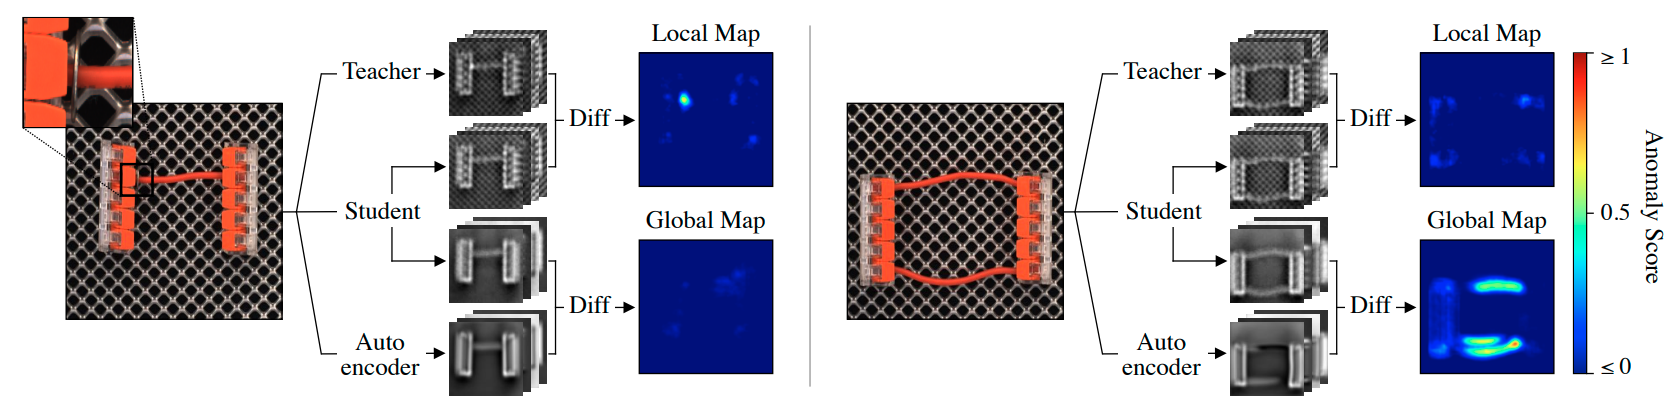
\includegraphics[width=0.8\textwidth]{bilder/localglobal.png}
    \caption{Veranschaulichung der Unterschiede zwischen lokaler und globaler Anomaliekarte. \cite{efficientad}}
    \label{fig:localglobal}
\end{figure}
Es handelt sich hierbei um zwei Beispielbilder aus dem bereits erwähnten Datensatz MVTec LOCO AD. Auf der linken Seite ist ein Testbild zu sehen, welches einen kleinen, strukturellen Defekt aufweist. \
Die globale Struktur des Bildes ist aber in Ordnung. Alle Baulteile sind an Stellen, an denen man sie erwarten würde.\
Dementsprechend ist die Differenz, die unten in der \glqq Global Map\grqq{} abgebildet ist, sehr gering. Dies lässt also keinen Schluss auf eine Anomalie zu.\
Die lokale Anomaliekarte hingegen, die oben zu sehen ist, zeigt eine deutlich erhöhte Differenz an der Stelle des Defekts, was wiederum eindeutig auf die tatsächlich\
existierende, strukturelle Anomalie hinweist.\\
Auf der rechten Seite ist ein Testbild zu sehen, welches eine logische Anomalie aufweist. Die globale Anomaliekarte zeigt hier eine deutlich erhöhte Differenz,\
während die lokale Anomaliekarte keine erhöhte Differenz aufweist.\\
Nun sollen aber nicht logische und strukturelle Anomlien voneinander unterschieden werden, sonder eine resultierende, finale Anomaliekarte soll erstellt werden.\
Dies geschieht, naheliegenderweise, durch eine Kombination der beiden Anomaliekarten.\ 
Es müssen allerdings unterschiedliche Rauschniveaus der beiden Anomaliekarten berücksichtigt werden, um keine falschen Positive zu erzeugen.\
Um das Ausmaße des Rauschens für beide Karten zu bestimmen, werden ungesehene Bilder aus dem Trainingsdatensatz verwendet. Mit diesen wird eine Menge\
aller auftretenden Differenzen jeweils für beide Karten bestimmt. Mithilfe dieser Mengen werden dann die Quantile $q_{a}$ und $q_{b}$ bestimmt, die das Rauschniveau der jeweiligen Karte beschreiben. \
Abschließend wird jeweils eine lineare Transformation bestimmt, die die den Wert $q_{a}$ auf 0 und den Wert $q_{b}$ auf \num{0,1} abbildet.\
Zu den einzelnen Zahlenwerten sind Ablation Studien in \cite{efficientad} zu finden.\\
Die finale Anomliekarte ergibt sich dann einfach aus der Addition der beiden Anomaliekarten.  
\section{Ergebnisse und Diskussion der Originalmethode}\label{subsec:efficientadergebnisseunddiskussion}
\textcolor{green}{\textit{Abgeschlossen: 02.11. v1}}\\
Trotz des leichtgewichtigen Aufbaus des PDNs, ist eine Beschleunigung der Feature Extraktion gegenüber einem kleinen ResNets nicht zu erwarten.\
Dies liegt vor allem daran, dass die Feature Maps in frühen Schichten des ResNets gegenüber dem Eingangsbild stark herunterskaliert werden. Zwar wird dies auch\
bei den hier verwendeten PDNs getan, aber in einer weniger stark ausgeprägten Weise.\
Bereits nach der \glqq Layer1\grqq{} ist bei einem ResNet, wie Abb. \ref{fig:ResNetPyramid} zu entnehmen ist, die räumliche Auflösung (Anzahl an Pixeln) $16$ mal kleiner als die des Eingangsbildes.\
Beim PDN wird sie durch ein Average-Pooling mit Kernelgröße $\texttt{k}=2$, Schrittweite $\texttt{s}=2$ lediglich um den Faktor $4$ reduziert.\
Weil somit der Tensor der Feature Maps, dessen Größe bei einem CNN maßgeblich die Anzahl an Berechnungen bestimmt, damit bei einem PDN deutlich größer ist,\
ist eine Beschleunigung der Feature Extraktion kaum zu erwarten.\ 
Der Vorteil eines solchen Ansatzes ist, dass die Auflösung der finalen Anomaliekarte auch ohne ein Hochskalieren verhältnismäßig groß bleibt.\
Insbesondere für eine Segmentierungsaufgaben ist das eine wertvolle Eigenschaft, die für diese Arbeit allerdings keine explizite Rolle spielt.\\
Vergleicht man die Laufzeiten gesamter ResNets aus Tab. \ref{tab:model-runtimes} mit denen der PDNs bestätigt sich die Vermutung, dass die Laufzeit\
nicht geringer als bei einem ResNet 18 oder 34 ist. Für ein Eingangsbild der Dimension $224\times 224$ ist die Laufzeit auf der Desktop-CPU (AMD Ryzen R5 5600X, mittlere Spalte)\
mit \num{42,42}\si{\milli\second} und \num{143,83}\si{\milli\second} für die kleine bzw. große Variante des PDNs sogar jeweils höher, als mit vergleichbaren ResNets.\
Auf der GPU hingegen (Nvidia RTX3060Ti, rechte Spalte), die das Mehr an Berechnungen durch Parallelisierung teilweise kompensieren kann, ist die Laufzeit\
mit \num{1,32}\si{\milli\second} bzw. \num{5,19}\si{\milli\second} im Falle der kleinen Variante des PDNs sogar geringer, als für ein ResNet 18 mit \num{1,46}\si{\milli\second}.\
An dieser Stelle ist allerdings zu erwähnen, dass je nach gewählter Hierarchieebene des ResNets, sich die Laufzeit für die Feature Extraktion verkürzt\
weil hintere Schichten des ResNets nicht mehr ausgeführt werden müssen. Hingegen entfällt der Einbettungsprozess, weil dieser bereits implizit im PDN integriert ist.\\
Betrachtet man die Laufzeiten des größereren PDNs, kann bereits jetzt festgestellt werden, dass lediglich das Verwenden des kleineren PDNs für diese Arbeit\
sinvoll ist. Die Laufzeit des größeren PDNs ist ohne Hardwarebeschleunigung schlicht zu hoch.\\
Wie bereits in der Einleitung zu diesem Kapitel erwähnt, ist EfficientAD eine sehr genaue und vielseitige Methode.\
Das Erkennen von logischen Anomlien ist zwar in dieser Arbeit nicht von Interesse, aber eines der Hauptziele in der Entwicklung von EfficientAD gewesen.\
Dass die Methode dennoch für strukturelle Anomalien sehr gut geeignet ist, zeigt sich in den Ergebnissen auf dem Datensatz MVTec AD.\
Diese Vielseitigkeit ist ein Alleinstellungsmerkmal von EfficientAD.\\
Eine Schwierigkeit, die von den Autoren, ähnlich wie bei SimpleNet, nicht genauer thematisiert wird, ist die Wahl eines Kriteriums, wann das Training beendet wird.\
Es wird im weiteren Verlauf dieses Kapitels gezeigt, dass dies einen großen Einfluss auf die erzielte Genauigkeit haben kann.\
Die Ergebnisse, die EfficientAD zur besten Methode auf dem Datensatz MVTec AD machen \cite{paperswithcode} beruhen auf einem nicht weiter spezifizierten\
\glqq Early Stopping\grqq{} Kriterium.\
Mutmaßlich handelt es sich dabei um eine fortlaufende Überwachung des Trainingsprozesses mithilfe eines Validierungsdatensatzes. Das beste Modell während des Trainingsprozesses\
wird dann als das finale Modell verwendet. Es stellt sich dann die Frage, wie dieser Validierungsdatensatz zustande kommt oder ob er dem Testdatensatz entspricht.\
Letztres wäre in gewisserweie eine Verletzung der wissenschaftlichen Integrität, weil der Testdatensatz dann nicht mehr unabhängig vom Trainingsprozess ist.\\
Wird auf das Early Stopping verzichtet, so kann das Training auch über die Anzahl an Iterationen gesteuert werden.\
Diese werden auf \num{70000} festgelegt. Die Ergebnisse, die dann erzielt werden, liegen für den Fall der Verwendung des größeren PDNs\
mit \num{99,1}\% gleichauf mit dem in \ref{sec:ErgebnisseUndDiskussionDerOriginalmethode} erzielten Ergebnissen. Für den kleineren PDN (S) ergibt sich eine immer noch guter\
durchschnittlicher AUROC von \num{98,8}\%.\
Nachfolgender Abschnitt zeigt, dass diese Ergebnisse plausibel sind.\\



\begin{figure}[h]
    \centering
    \input{tikz/esmalledited}
    \caption{Laufzeiten für EfficientAD S.}
    \label{fig:efficientadlaufzeitensmall}
\end{figure}
% \section
% $$
% \mathcal{L} %= \frac{\sum_{c}\lVert A(x)_{c} \rVert^{2}_{F}}{HWC}
% $$
      % -*- TeX -*- -*- DE -*-

\chapter{SimpleNet}\label{ch:SimpleNet}
Hier dann SimpleNet....

      \appendix
      % -*- TeX -*- -*- DE -*-

\chapter{ASCII-Tabelle}

\dots



\backmatter

%%>> nur wenn option:biblatex NICHT gesetzt
			\bibliography{referenzen}
%%<< nur wenn option:biblatex NICHT gesetzt

%%%>> nur wenn option:biblatex gesetzt
%% Achtung: BibTeX command has to be 
%%		biber.exe "%bm" -q
%% now, where %bm is the full path of main file name without extension
%\selectlanguage{ngerman}
%\printbibliography[heading=bibintoc]
%%<< nur wenn option:biblatex gesetzt
\end{document}
